\documentclass[%
reprint,
superscriptaddress,
%groupedaddress,
%unsortedaddress,
%runinaddress,
%frontmatterverbose,
%preprint,
showpacs,preprintnumbers,
%nofootinbib,
%nobibnotes,
%bibnotes,
amsmath,amssymb,
aps,
%pra,
%prb,
prd,
%prl,
%rmp,
%prstab,
%prstper,
%floatfix,
]{revtex4-1}

\usepackage{float}
\usepackage{graphicx}% Include figure files
\usepackage{dcolumn}% Align table columns on decimal point
\usepackage{bm}% bold math
\usepackage{bbold}
\usepackage{braket}
\usepackage{amssymb,amsmath}


\usepackage{color}
%\usepackage[dvipsnames, svgnames, x11names]{xcolor}
\usepackage{amsfonts}
\usepackage{subfigure}
\usepackage{array}


\newcommand{\Tr}{\ensuremath{\operatorname{Tr}}}
\newcommand{\tr}{\ensuremath{\operatorname{tr}}}
\newcommand{\Omegaqq}{\ensuremath{\Omega_{\bar{q}q}}}
\newcommand{\vev}[1]{\ensuremath{\left\langle #1 \right\rangle}}
\newcommand{\einh}[1]{\ensuremath{\,\text{#1}}}
\newcolumntype{L}{>{\centering\arraybackslash}m{3cm}}



\newcommand{\overbar}[1]{\mkern 1.5mu\overline{\mkern-1.5mu#1\mkern-1.5mu}\mkern 1.5mu}



% color def's

\definecolor{blue}{rgb}{0,0,1}
\newcommand{\colb}[1]{{\color{blue} #1}}
\definecolor{green}{rgb}{0,1,0}
\newcommand{\colg}[1]{{\color{green} #1}}
\definecolor{red}{rgb}{1,0,0}
\newcommand{\colr}[1]{{\color{red} #1}}
\newcommand{\colJ}[1]{{\color{cyan} #1}}
\definecolor{gray}{rgb}{.5,.5,.5}
\newcommand{\drop}[1]{{\sout{ {\color{gray} #1}}}}
\definecolor{darkgreen}{rgb}{.0,.5,.0}
\newcommand{\colL}[1]{{\color{darkgreen} #1}}


% units and refs
\usepackage{xspace}
\usepackage{siunitx}
\usepackage{xfrac}
\usepackage{hyperref}
\usepackage[nameinlink]{cleveref}
\usepackage{appendix}
\usepackage{units}
% other
\usepackage{xifthen}
\usepackage{xcolor}
\hypersetup{
	colorlinks,
	linkcolor={red!75!black},
	citecolor={blue!75!black},
	urlcolor={blue!75!black}
}
%%%%%%%%%%%%%%% Refs %%%%%%%%%%%%%%%%%%%%%%%%%%%
\def\Fig#1{\Cref{#1}} 
\def\Figs#1{\Cref{#1}} 
\def\fig#1{\Cref{#1}}

\def\Tab#1{\Cref{#1}}
\def\tab#1{\Cref{#1}}

\def\Eqs#1{\Cref{#1}}
\def\Eq#1{\Cref{#1}}
\def\eq#1{\Cref{#1}}
\def\eqref#1{\Cref{#1}}

\def\sec#1{\Cref{#1}}
\def\app#1{\hyperref[#1]{App.~\ref{#1}}}
\def\app#1{\Cref{#1}}

\renewcommand{\tableautorefname}{Tab.} 
\renewcommand{\equationautorefname}{Eq.} 
%%%%%%%%%%%%%%%%%%%%%%%%%%%%%%%%%%%%%%%%

\newcommand{\Phibar}{\ensuremath{\bar{\Phi}}}
\newcommand{\LPQM}{\ensuremath{\mathcal{L}_{\textrm{PQM}}}\xspace}

\def\dbar{{\mathchar'26\mkern-12mu d}}
\def\lA0{{\langle A_0 \rangle}}
\def\bA0{{\bar{A}_0}}
\def\lLA{{\langle L[A_0] \rangle}}
\def\lL{{\langle L \rangle}}
\def\lLc{{\langle L^\dagger \rangle}}
\def\lLAc{{\langle L^\dagger[A_0] \rangle}}


\def\dr{{D\!\llap{/}}\,}
\def\Dr{{D\!\llap{/}}\,}
\def\ipv{\vec{p}\llap{/}}
\def\pslash{p\llap{/}}

\def\0#1#2{\frac{#1}{#2}}

\newcommand{\bsig}{\ensuremath{\bar{\sigma}}}
\newcommand{\lsm}{L\ensuremath{\sigma}M\xspace}
\newcommand{\pT}{\ensuremath{T_0}}
\newcommand{\Tl}{\ensuremath{T_\chi}}
\newcommand{\Ts}{\ensuremath{T_\chi^s}}
\newcommand{\Tchi}{\ensuremath{T_\chi}}
\newcommand{\Td}{\ensuremath{T_d}}
\newcommand{\Tc}{\ensuremath{T_c}}
\newcommand{\muc}{\ensuremath{\mu_c}}
\newcommand{\coloronl}{(color online)\xspace}

\newcommand{\mrm}[1]{\mathrm{#1}}
\def\qbar{\bar{q}}
\newcommand{\sx}{\sigma_{x}}
\newcommand{\sy}{\sigma_{y}}

%%%%%%%%%%%%% Hypersetup %%%%%%%%%%%%%

\newcommand{\gettitle}{Baryon number fluctuations at finite temperature and density in QCD}

\renewcommand{\figureautorefname}{Fig.}
\renewcommand{\sectionautorefname}{Sec.}
\renewcommand{\subsectionautorefname}{Subsec.}
\renewcommand*{\appendixautorefname}{App.}


%%%%%%%%%%%%%% for corrections %%%%%%%%%%%
\newcommand{\colwj}[1]{\textcolor{blue}{#1}}
\newcommand{\colxf}[1]{\textcolor{cyan}{#1}}
\newcommand{\cJMP}[1]{\textcolor{red}{#1}}
\newcommand{\colfab}[1]{\textcolor{magenta}{#1}}
\newcommand{\colrui}[1]{\textcolor{green}{#1}}
\newcommand{\colshi}[1]{\textcolor{Plum}{#1}}

%
%%%%%%%%%%%%%%%%%%%%%%%%%%%%%%%%%%%%%%%%%%%%%%%%%%%%%%%%%%%%%%%%%%%%%%%%%%%%%

\graphicspath{{./figures/}{./}}

\begin{document}
%\preprint{}
	
\title{Baryon number fluctuations at finite temperature and density in QCD}
	
	

\author{Wei-jie Fu}
\affiliation{School of Physics, Dalian University of Technology, Dalian, 116024,
		P.R. China}

\author{Jan M. Pawlowski}
\affiliation{Institut f\"ur Theoretische Physik, Universit\"at Heidelberg, Philosophenweg 16, 69120 Heidelberg, Germany}
	\affiliation{ExtreMe Matter Institute EMMI, GSI, Planckstra{\ss}e 1, D-64291 Darmstadt, Germany}
	
\author{Fabian Rennecke}
\affiliation{Brookhaven National Laboratory, Upton, NY 11973, USA}
	
\author{Rui Wen}
\affiliation{School of Physics, Dalian University of Technology, Dalian, 116024,
		P.R. China}
	
\author{Shi Yin}
\affiliation{School of Physics, Dalian University of Technology, Dalian, 116024,
		P.R. China}
	
	
\begin{abstract}
Fluctuations of conserved charges have been calculated at finite temperature and finite density. 
\end{abstract}

\maketitle

	
\section{Introduction}\label{sec:int}

Fluctuations plays an important role in finding the CEP.
	
	
%%%%%%%%%%%%%%%%%%%%%%%%%%%%%%%%%%%%%%%%%%%%%%%%%%%%%%%%%%%%%%%%%%%%%%%%%%%%%%%%%%%%%%%%%%%%%%%%%%%%%%%%%%%%%%%%%%%%%%%
	
\section{2+1 flavors QCD  theories}
\label{sec:FRG}
	
%
%%%%%%%%%%%%%%%%%%%%%%%%%%%%
\begin{figure}[t]
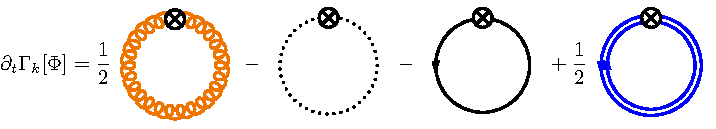
\includegraphics[width=0.45\textwidth]{QCD_equation}
\caption{Diagrammatic representation of the QCD flow equation. The lines stand for the full propagators of gluon, ghost, quark, and mesons, respectively. The arrows in quark and meson lines indicate the quark number (baryon number) flow. The crossed circles represent the infrared regulators.}\label{fig:QCD_equation}
\end{figure}
%%%%%%%%%%%%%%%%%%%%%%%%%%%%%
%

\subsection{The effective action}\label{sec:effective_action}

The  Euclidean  scale-dependenteffective  action $\Gamma_k$ for $N_f=2+1$ flavors are given as 
\begin{align}
\Gamma_k&=\int_x\bigg \{ \frac{1}{4} F_{\mu\nu}^a F_{\mu\nu}^a+Z_c (\partial_\mu \bar c^a) D_{\mu}^{a b} c^{b}+\frac{1}{2\xi}(\partial_\mu A_{\mu}^{a})^2\\ \nonumber
&+\frac{1}{2}\int_p A^a_{\mu}(-p) ({\Gamma_{AA}^{(2)}}_{\mu \nu}^{ab}-Z_A \Pi_{\mu \nu}^{\perp}\delta^{ab} p^2)A _{\nu}^b(p)\\  \nonumber
&+\bar q [Z_q (\gamma_\mu D_\mu-\gamma_0(\hat \mu+ig A_0)]q \\  \nonumber
&-\lambda_q \sum_{a=0}^8 [(\bar q T_a  q)^2+(\bar q i \gamma _5 T_a q)^2]\\  \nonumber
&+\bar q  h^{1/2}  \cdot \Sigma_{5} \cdot h^{1/2} q+tr \big (Z_{\Sigma}^{1/2} \cdot \partial_\mu\Sigma \cdot Z_{\Sigma}^{1/2}\cdot \partial_\mu\Sigma^\dagger\bigr)  \\  \nonumber
&+\tilde U_k(\Sigma,\Sigma^\dagger)+V_{glue}(L,\bar L)
\bigg \}\label{}
\end{align}
with $\int_x=\int_0^{\frac{1}{T}} d x_0 \int d^3 x$. All couplings and wave function renormalisations are depend on the RG scale k.  

\textcolor{red}{The gluon sector}

The nonets of scale and pseudoscale meson field are define as 
\begin{align}
  \Sigma&=T^a(\sigma^a+i \pi^a)\,. \quad (a=0,1,...,8)
\end{align}
with $T^a=\lambda^a/2(a=1,...,8)$ and $T^{0}=\frac{1}{\sqrt{2N_{f}}}\mathbb{I}_{N_{f}\times N_{f}}$ are generators of $SU(N_f=3)$, and  $\lambda^a$ are  Gell-Mann matrices.  $\sigma^a$ and $\pi^a$ mean the scalar and pseudoscalar fields, respectively.  The meson fields are coupled with quarks through a Yukawa term with
\begin{align}\label{}
  \Sigma_5&=T^a(\sigma^a+i \gamma_5 \pi^a)\,. \quad (a=0,1,...,8)
\end{align}
where Yukawa coupling is also a matrice
\begin{align}
h=\begin{pmatrix} 
h_{l}&0&0\\
0&h_{l}&0\\
0&0&h_{s}
\end{pmatrix}
\end{align}
the subscript $l/s$ denote light or strange Yukawa coupling. 

The meson effective potential can be devided into three parts
\begin{align}
  \tilde{U}_{k}(\Sigma,\Sigma^\dagger)&=U_k(\rho_1,\rho_2)-c_A \xi-c_l\sigma_l-c_s\sigma_s\,, \label{eq:tildeU}
\end{align}
here $U_k(\rho_1,\rho_2)$ is an arbitrary function of chiral symmetry invariant variables $\rho_1,\rho_2$.  $ c_A \xi$ is Kobayashi-Maskawa-’t Hooft trem which breaks $U_A(1)$ symmetry. The last two terms of Eq.(\ref{eq:tildeU}) are linear sigma terms, which break the chiral symmetry. The $\rho_1,\rho_2$ are defined as:
\begin{align}
\rho_1&=\text{tr}(\Sigma \cdot \Sigma ^\dagger) \\
\rho_2&=\sqrt{6 \cdot \text{tr}\bigg (\Sigma \cdot \Sigma ^\dagger-\frac{1}{3} \rho_1 \mathbb{I}_{3 \times 3} \bigg )^2 }
\end{align}
We solve the effective potential  by Taylor expaned method, for more details, see appendix.

In this work, we don't distinguish the light and strange quark wave function renormalisations, i.e. $Z_q\simeq Z_l$ and all mesons have the same wave function renormalisations,  for simplicity. In 
2+1 flavors quark meson model \cite{Rennecke:2016tkm} , $Z_\Sigma=Z_{\pi^+}$ , and we also employ this assumption.

The quark masses are given as :
 \begin{align}\label{quarkmass_eq}
m_l=\frac{h_{l}}{2}\sigma_l , \quad m_s=\frac{h_{s}}{\sqrt{2}}\sigma_s
\end{align}
And the meson mass squares are given from the Hessian matrix of the meson effective potential, i.e.
 \begin{align}
H_{ij}=\frac{ \partial^2 \tilde{U}_{k}(\Sigma,\Sigma^\dagger)}{\partial \phi_i \partial \phi_j}
 \end{align}
see appendix and work \cite{Rennecke:2016tkm,Wen:2018nkn} for more details.

%%%%%%%%%%%%%%%%%%%%%%%%%%%%%%%%%%%%%%%%%%%%%%%%%%%%%%%%%%%

\subsection{Flow equations}\label{sec:Floweq}

%
%%%%%%%%%%%%%%%%%%%%%%%%%%%%
\begin{figure}[t]
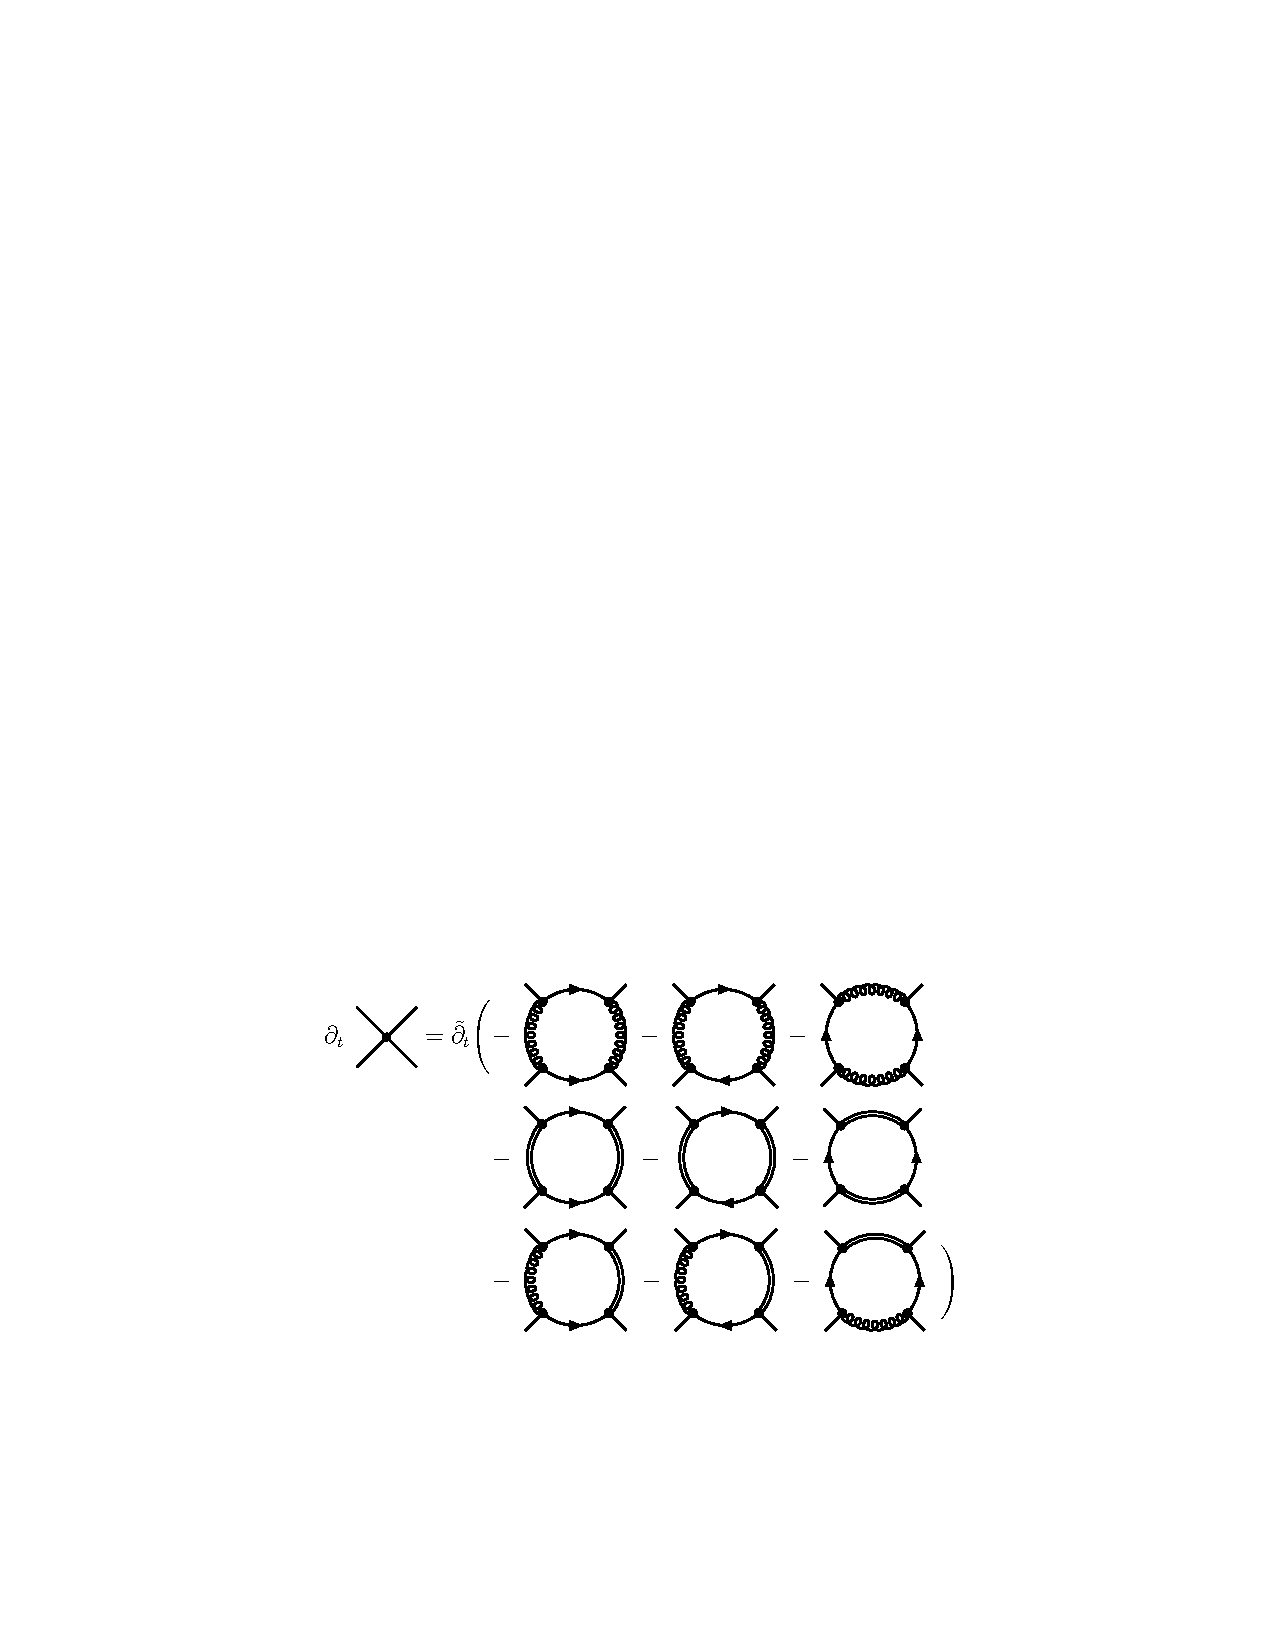
\includegraphics[width=0.45\textwidth]{4quark}
\caption{Flow equation for the four-quark coupling.}\label{fig:4quark}
\end{figure}
%%%%%%%%%%%%%%%%%%%%%%%%%%%%%
%

The meson fields are composite condensate fields from QCD theories. So we need empoly the Wetterich equation with dynamical hadronisation\cite{Fu:2019hdw}, which reads 
\begin{align}\label{Wettericheq}
&\partial_t \Gamma_k[\Phi]+\int \langle  \partial_t  \hat \phi_{k,i}\rangle \bigg ( \frac{\delta \Gamma_k [\Phi]}{\delta \phi_i}+c_\sigma \delta_{i \sigma}\bigg ) \\ \nonumber
&=\frac{1}{2} \text{Tr}(G_k[\Phi] \partial_t R_k)+\text{Tr}\bigg( G_{\phi \Phi_j} [\Phi] \frac{\delta \langle  \partial_t  \hat \phi_{k,i}\rangle}{\delta \Phi_j } R_{\phi} \bigg) 
\end{align}
We distinguish the light and strange dynamical hadronisation, which reads
\begin{align}
\langle  \partial_t  \hat \phi_{k}\rangle&= [(\bar q \dot{\pmb{A} }_{k}^{\frac{1}{2}} T_a  \dot{\pmb{A} }_{k}^{\frac{1}{2}}   q)+(\bar q \dot{\pmb{A} }_{k}^{\frac{1}{2}} i \gamma _5 T_a \dot{\pmb{A} }_{k}^{\frac{1}{2}} q)]+\dot{B}_k \Sigma
\end{align}
here $\dot{\pmb{A} }_{k}$ is also a diagonal matrice
\begin{align}
\dot{\pmb{A} }_{k}=\begin{pmatrix} 
\dot{A}_{l,k}&0&0\\
0&\dot{A}_{l,k}&0\\
0&0&\dot{A }_{s,k}
\end{pmatrix}
\end{align}
As pointed out in ref \cite{Braun:2014ata, Fu:2019hdw} , we choose $\dot{B}_k =0$.
For convenience, we introduce light and strange matrices $T^L$ and $T^S$, see appendix.
By taking secomd derivative of of each side of \Eq{Wettericheq}, we get
\begin{align}
- \partial_t \lambda_q + \dot{A}_{a,k} h_{k}=-\text{Flow} _{(\bar q T^a q) (\bar q T^a q)}^{(4)}
\quad \text{for} \quad a=L,S 
\end{align}
Here, $\text{Flow} _{(\bar q T^a q) (\bar q T^a q)}^{(4)}$ denotes four-quark coupling flow equation, which is depicted by \fig{fig:4quark}. With the fully hadronised condication
\begin{align}\label{lambda_eq}
\lambda_q  \equiv 0 , \quad \forall k
\end{align}
we get the hadronisation function
\begin{align}
\dot{A}_{l,k}=-\frac{1}{ h_{l,k}} \text{Flow}_{(\bar q T^L q) (\bar q T^L q)}^{(4)} \\
\dot{A}_{s,k}=-\frac{1}{ h_{s,k}}  \text{Flow}_{(\bar q T^S q) (\bar q T^S  q)}^{(4)}
\end{align}
For the yukawa couplings, we take derivative of of each side of \Eq{Wettericheq} and project it on light or strange part, we get
\begin{align}
\partial \bar h_{l,k}&=\bigg( \eta_{l,k} +\frac{1}{2}\eta_{\phi,k}\bigg ) \bar h_{l,k}-\frac{1}{\bar \sigma_L} \frac{\delta \bar{\tilde U}(\Sigma)}{\delta \bar \sigma_L}\dot{\bar A}_{l,k}+\frac{1}{\bar \sigma_L} \text{Re} \overline{  \text{Flow} }_{(\bar q T^L q)}^{(2)}\\
\partial \bar h_{s,k}&=\bigg( \eta_{s,k} +\frac{1}{2}\eta_{\phi,k}\bigg ) \bar h_{s,k}-\frac{1}{\bar \sigma_S} \frac{\delta \bar{\tilde U}(\Sigma)}{\delta \bar \sigma_S}\dot{\bar A}_{s,k}+\frac{1}{\bar \sigma_S} \text{Re} \overline{  \text{Flow} }_{(\bar q T^S q)}^{(2)} \label{Yukawa_eq}
\end{align}
%%%%%%%%%%%%%%%%%%%%%%%%%%%%%%%%%%%%%%%%%%%%%%%%%%%%%%%%%%%%%%%%%%%%%%%%%%

	
\section{Numerical results}
\label{sec:result}

%
%%%%%%%%%%%%%%%%%%%%%%%%%%%%%
\begin{figure*}[t]
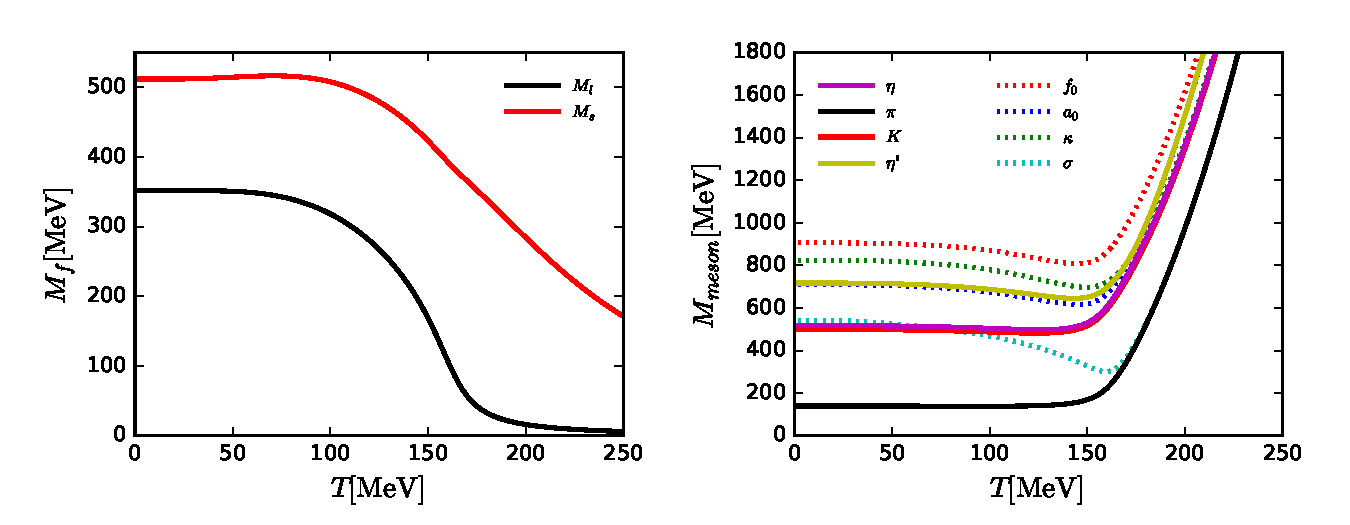
\includegraphics[width=0.9\textwidth]{MFMBO}
\caption{The quark (left panel) and  meson masses (right panel) as function of temperature at vanished chemical potentional. The solid and dashed lines in right panel correspond to scale and pseudoscale meson fields, respectively.}\label{fig:MFMBO}
\end{figure*}
%%%%%%%%%%%%%%%%%%%%%%%%%%%%%
%

\subsection{Numerical setup and Chiral condensates}
We choose the UV cutoff $\Lambda=20$GeV.

In \fig{fig:MFMBO} left panel, we show the light and strange quark masses as function of temperature at vanished chemical potentional. At T=0, we set $m_l=350$MeV and $m_s=510$MeV. At high temperatre, the chiral symmetry is restore, the light quark mass trend to zero. The pseudo critical temperature is around $150$ MeV, however a precise definition given by quark condensate will be given later. In \fig{fig:MFMBO} right panel, we show the masses of the nonets of scale and pseudoscale meson as function of temperature. The solid and dashed lines correspond to scale and pseudoscale meson fields, respectively. $\pi-\sigma$, $\eta' - a_0$, $\kappa-K$ are the chiral partners, which become degenerate with each other at high temperature. This  have been observed in low energy effective model \cite{Schaefer:2008hk,Tiwari:2013pg,Rai:2018ufz,Mitter:2013fxa,Rennecke:2016tkm,Wen:2018nkn}. One interesting thing is that in our theory, $\eta' - a_0$ are chiral partner, which is same with quark-meson model in mean-field approximation \cite{Schaefer:2008hk,Tiwari:2013pg,Rai:2018ufz} and LPA truncation\cite{Mitter:2013fxa,Rennecke:2016tkm,Wen:2018nkn} , rather than $\eta - a_0$, which is observed in quark-meson model beyond LPA truncation in  \cite{Rennecke:2016tkm}. This is related with the axial anomaly and the pseudoscalar mixing anglea, a thorough analysis see  \cite{Rennecke:2016tkm}. Compared with the low energy effective theory, meson masses in QCD increase faster at high temperature and the meson fileds decouple faster from the the systerm. This also consist with the result that the QCD chiral symmetry restore is stronger than the LEEF.

The chiral condensates are defined as
\begin{align}
\Delta_{q_i}=m_{q_i}^0\frac{T}{\mathcal{V}}\int_x\langle \bar q_i(x)q_i(x)\rangle
\end{align}
The renormalised condensate 
\begin{align}\label{eq:DeltaR}
\Delta_{q_i,R}=\frac{1}{\mathcal{N}_R}[\Delta_{q_i}(T,\mu_q)-\Delta_{q_i}(0,0)]
\end{align}
with $\mathcal{N}_R$ is a normalised constant.
The reduced condensate \cite{Herbst:2013ufa, Fu:2019hdw} 
\begin{align}\label{eq:Deltals}
\Delta_{l,s}&\equiv\frac{\Delta_{l}(T,\mu_B)-\Big( \frac{m_l^0}{m_s^0} \Big)^2 \Delta_s(T,\mu_B)}{\Delta_{l}(0,0)-\Big( \frac{m_l^0}{m_s^0} \Big)^2 \Delta_s(0,0)}\\
&=\frac{\sigma_{l}(T,\mu_B)-\big( \frac{c_l}{c_s} \big) \sigma_s(T,\mu_B)}{\sigma_{l}(0,0)-\big( \frac{c_l}{c_s} \big) \sigma_s(0,0)}
\end{align}
In \fig{fig:Delta}, we plot the renormalised light chiral condensate $\Delta_{l,R}$ and  the reduced condensate $\Delta_{l,s}$ as functions of temperature  at vanished chemical potential. We compare with former work \cite{Fu:2019hdw}  and the lattice calculation \cite{Borsanyi:2010bp}. The the normalisation $\mathcal{N}_R$ in \Eq{eq:DeltaR} are same with the former work \cite{Fu:2019hdw}. Here we only choose the constituent quark mass $\Delta \bar m _{sl}=\bar m_s-\bar m_l=150$ MeV results in \cite{Fu:2019hdw}, which the ratios of current quark mass $m_s^0/m_l^0=27$,   as comparison. Notable, in this work,  the ratios of current quark mass $m_s^0/m_l^0=c_s/c_l$ is also choose as 27 and the constituent quark mass are selfconsistent calculated in this work. \fig{fig:Delta} show our results consistent well with the former work \cite{Fu:2019hdw}  and the lattice calculation \cite{Borsanyi:2010bp}, which imply the pseudo critical temperature is also in agreement with them.

%
%%%%%%%%%%%%%%%%%%%%%%%%%%%%%
\begin{figure*}[t]
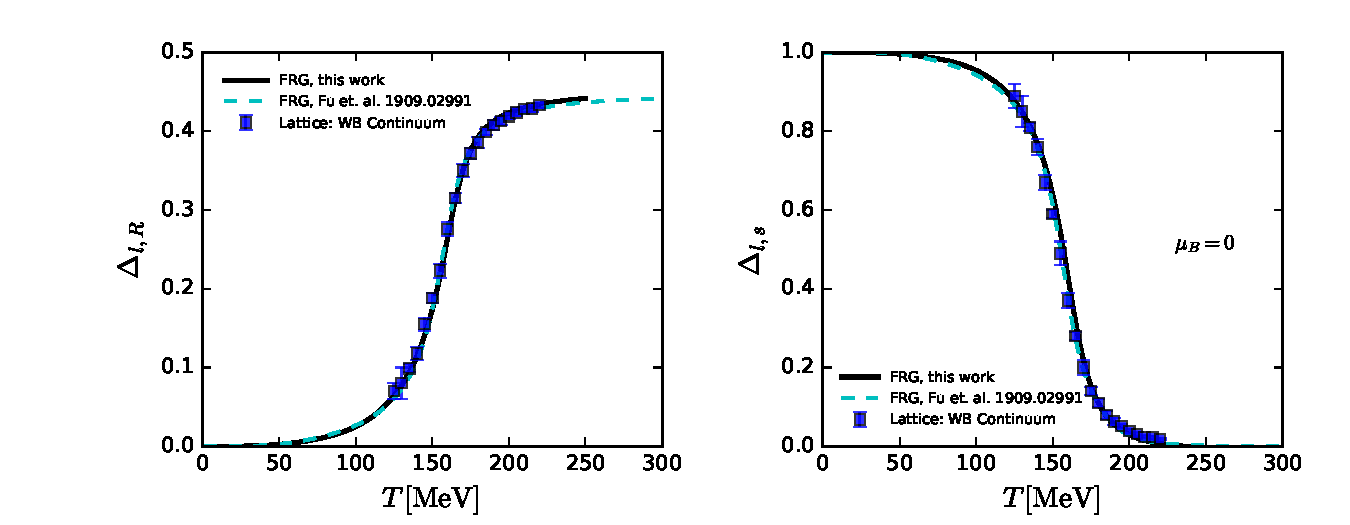
\includegraphics[width=0.95\textwidth]{Delta}
\caption{The renormalised light chiral condensate $\Delta_{l,R}$ (left panel) and  the reduced condensate $\Delta_{l,s}$ (right panel) }\label{fig:Delta}
\end{figure*}
%%%%%%%%%%%%%%%%%%%%%%%%%%%%%
%

\subsection{Baryon number fluctuations at vanishing density}

The pressure are given from the grand potential
\begin{align}
p=\Omega(0,0)-\Omega(T,\mu)
\end{align}
with 
\begin{align}
\Omega(T,\mu)=\tilde{U}_{k}(\Sigma,\Sigma^\dagger)+U_{glue}(L,\bar L)
\end{align}
and the generalised susceptibilities of the baryon number are obtain from derivatives of the pressure
\begin{align}
\chi_n^B=\frac{\partial^n}{\partial (\hat \mu_B)^n}\frac{p}{T^4}
\end{align}
with $\hat \mu_B\equiv \mu_B/T$
and the ratio between the n-th and m-th oder of the generalised susceptibilities are bdfined by
\begin{align}
R^B_{nm}=\frac{\chi_n^B}{\chi_m^B}
\end{align}


%%%%%%%%%%%%%%%%%%%%%%%%%%%%%
\begin{figure*}[t]
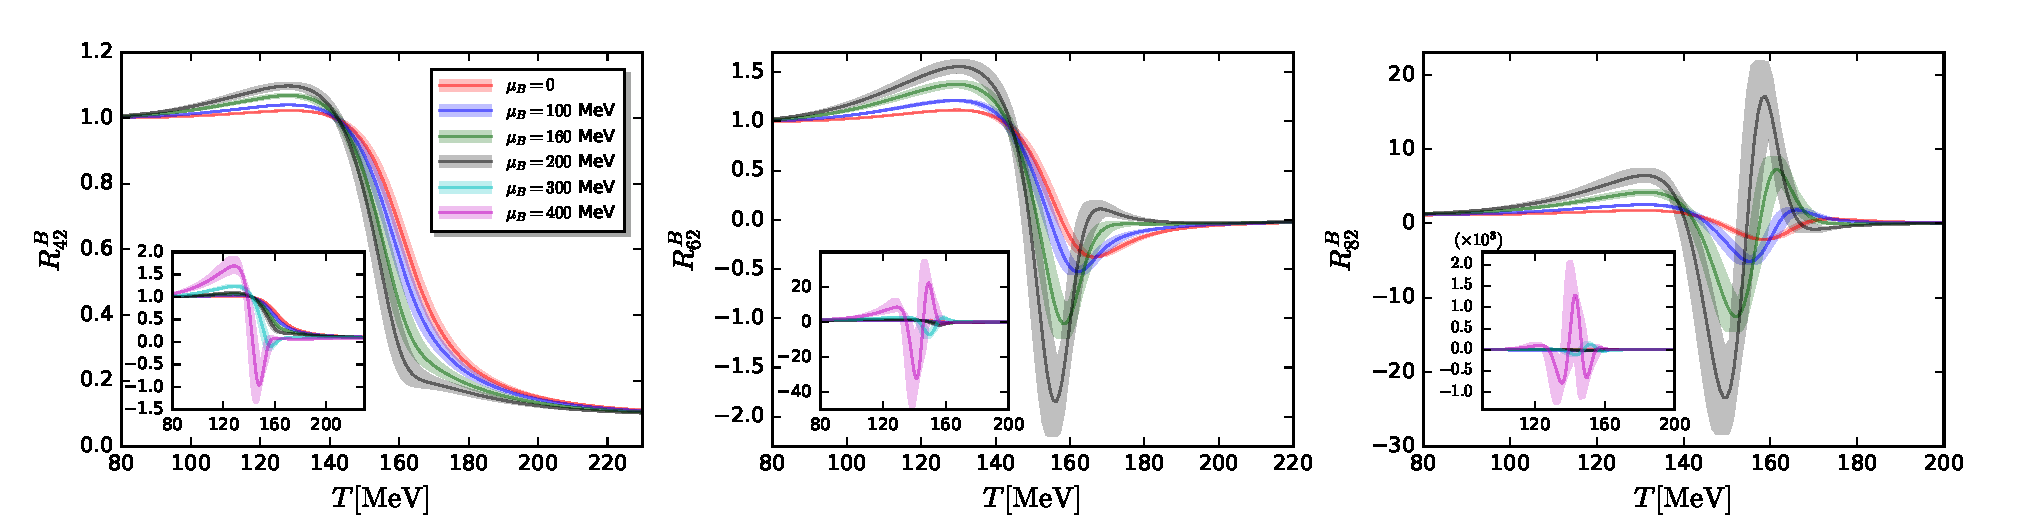
\includegraphics[width=1.\textwidth]{R42R62R82-T-muB0to400}
\caption{$R^{B}_{42}$ (left panel), $R^{B}_{62}$ (middle panel), and $R^{B}_{82}$ (right panel) as functions of the temperature at several values of $\mu_B$. Insets in each plot show their respective zoomed-out view. }\label{fig:R42R62R82-T-muB0to400}
\end{figure*}
%%%%%%%%%%%%%%%%%%%%%%%%%%%%%
%


%%%%%%%%%%%%%%%%%%%%%%%%%%%%%%%%%%%%%%%%%%%%%%%%%%%%%%%%%%%%%
\section{Numerical results and discussions}
\label{sec:num}

In this section we present and discuss our numerical results for hyper-order fluctuations on the freeze-out curve. At vanishing chemical potential the lower orders are compared to results from lattice calculations. We then discuss the implications of our predictions for the hyper-order baryon number fluctuations for decreasing collision energies (increasing chemical potential) for heavy-ion collision experiments. 

%%%%%%%%%%%%%%%%%%%%%%%%%%%%%%%%%%%%%%%%%%%%%%%%%%%%%%%%%%%%%

\subsection{Hyper-order baryon number fluctuations at vanishing density: benchmarks and predictions}
\label{subsec:hyper-order0}

We start our discussion of the numerical results in our QCD-assisted low-energy effective theory with benchmark results at vanishing chemical potential, $\mu_B=0$. We have already seen in \sec{subsec:scale} that the fourth order fluctuations $R^B_{42}$, \Eq{eq:Rnm}, agrees quantitatively with the respective lattice result, see \fig{fig:T-adjust} and \fig{fig:R42R62R82-T-muB0}, left panel. We emphasise again  that the thermal dependence of $R^B_{42}$ is a prediction of the present LEFT. Now we also compare the temperature dependence of the hyper-fluctuations $R^B_{62}$ and $R^B_{82}$ with the corresponding lattice results in the middle and right panels of \Fig{fig:R42R62R82-T-muB0}, respectively. We depict both our numerical results and lattice results from the HotQCD collaboration, \cite{Bazavov:2017dus,Bazavov:2017tot,Bazavov:2020bjn}, and the Wuppertal-Budapest collaboration, \cite{Borsanyi:2018grb}. 

With the increase of the order of fluctuations, the uncertainties of lattice results increase significantly. Moreover, the eighth-order fluctuations $R^{B}_{82}$ obtained by the two collaborations show a significant quantitative difference, although their form is qualitatively consistent with each other. 

The hyper-order baryon number fluctuations computed in the current setup are in qualitative agreement with both lattice results. However, our results single out the lattice results of the Wuppertal-Budapest collaboration, with which we observe quantitative agreement. This situation is very reminiscent of the pressure prediction in \cite{Herbst:2013ufa}: similarly to the current situation with lattice predictions of hyper-fluctuations, the pressure predictions of the lattice collaborations had not converged yet. A less advanced version of the current QCD-assisted LEFT framework then predicted the correct pressure result. 
We have also computed the hyper-order fluctuations within a simple hadron resonance gas model \cite{BraunMunzinger:2003zd}. Essentially, they are all constant with only a very minor monotonic increase with $T$ for $T \lesssim 140$~MeV, starting from unity at $T=0$. This is in quantitative agreement with our findings at low temperatures. In summary, the current setup passes all benchmark tests quantitatively and provides the full temperature-dependence of hyper-fluctuations. We have also computed even higher order baryon number fluctuations. In \Fig{fig:R102-T-muB0} we show our result for the temperature-dependence of the tenth order ratio $R^{B}_{10\,2}=\chi^{B}_{10}/\chi^{B}_{2}$ at vanishing chemical potential, $\mu_B=0$. So far no lattice results for the tenth-order fluctuation are available, and the dependence of $R^{B}_{10\,2}$ on the temperature in \Fig{fig:R102-T-muB0} is  a prediction by the current QCD-assisted LEFT and awaits confirmation by other calculations, e.g., lattice QCD, in the future.

%
%%%%%%%%%%%%%%%%%%%%%%%%%%%%%
\begin{figure*}[t]
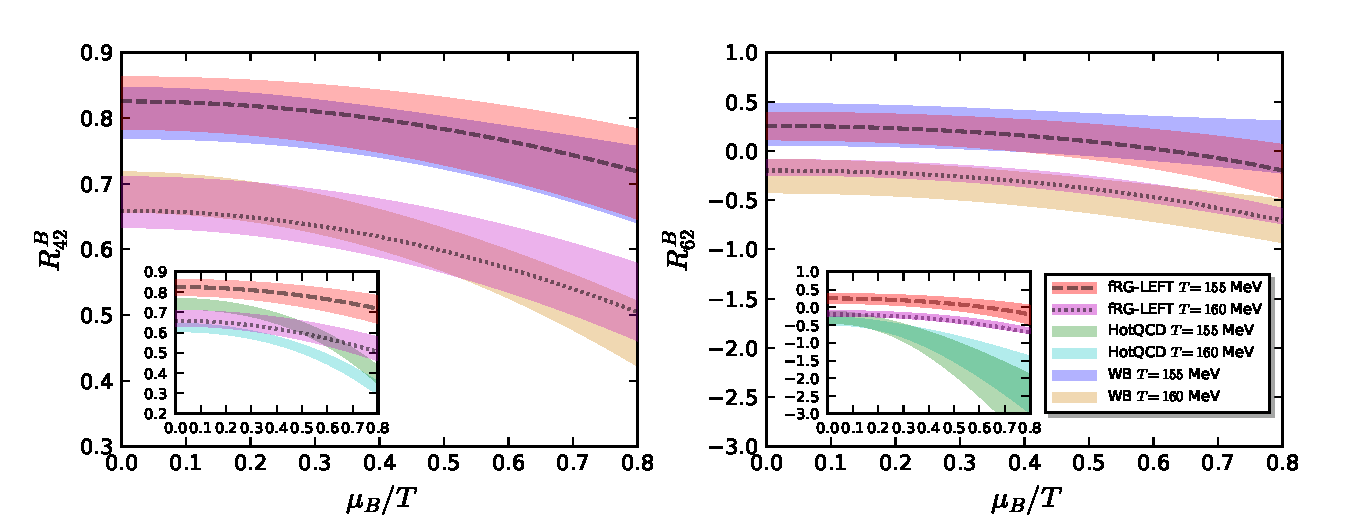
\includegraphics[width=0.9\textwidth]{R42R62-muBoT}
\caption{$R^{B}_{42}$ (left panel) and $R^{B}_{62}$ (right panel) as functions of $\mu_B/T$ with $T=155$ MeV and $T=160$ MeV from the eighth-order Taylor expansion in $(\mu_B/T)^2$ around vanishing $\mu_B$ shown in \Eq{eq:chiBTay}. Our results from the QCD-assisted LEFT are  compared to those from lattice QCD by the HotQCD collaboration \cite{Bazavov:2020bjn} and the Wuppertal-Budapest collaboration \cite{Borsanyi:2018grb}. We show the comparison to HotQCD in the inlays, as these results deviate considerably from both ours and the WB results.}\label{fig:R42R62-muBoT}
\end{figure*}
%%%%%%%%%%%%%%%%%%%%%%%%%%%%%
%

%%%%%%%%%%%%%%%%%%%%%%%%%%%%%%%%%%%%%%%%%%%%%%%%%%%%%%%%%%%%%%%

\subsection{Hyper-order baryon number fluctuations at finite  density}
\label{subsec:hyper-ordermuB}
With successfully passing the benchmark tests, we proceed with the results for baryon number fluctuations at finite chemical potential. This will allow us to finally compare the theoretical predictions on the freeze-out curve with the experimental measurements in \sec{subsec:freezout}. 

Equally relevant is the self-consistent evaluation of the reliability of a Taylor expansion in baryon-chemical potential that underlies the extension of lattice results at vanishing chemical potential to $\mu_B\neq 0$. This is particularly important for predictions of the location of the critical endpoint based on such an expansion. Here we can investigate the convergence of the Taylor expansion around $\mu_B = 0$ by comparison to our direct computation at finite $\mu_B$.

First we investigate the temperature-dependence of the baryon number fluctuations for different chemical potentials. This also allows us to discuss the reliability bounds of the current LEFT-setup for increasing chemical potential. In \Fig{fig:R42R62R82-T-muB0to400} we show the temperature-dependence of the ratios $R^{B}_{42}$, $R^{B}_{62}$ and $R^{B}_{82}$ for chemical potentials $\mu_B=0, 100, 160, 200, 300, 400$. First, we note that at small temperatures the thermodynamic properties of the QCD medium are well described by a dilute gas of hadrons, where the net-baryon number follows a Skellam distribution. Thus, all ratios approach unity at vanishing temperature. At very large temperature the system is governed by asymptotically free quarks, where fluctuations are only Gaussian. Hence, $R^{B}_{n2}$ goes to zero for all $n>2$ at large $T$. Consequently, the non-trivial behaviour of the fluctuations between these two limiting cases shown in \Fig{fig:R42R62R82-T-muB0to400} is directly related to the crossover from the hadronic- to the quark-gluon regime of QCD. The magnitude, but also the error of the fluctuations grow with increasing chemical potential. Both effects are more pronounced for higher order fluctuations. The increase in magnitude is directly linked to the sharpening of the chiral crossover with increasing chemical potential, cf.\ \fig{fig:QCD-scalematching}. We expect that the current LEFT-setup is gradually loosing its predictive power for fluctuations on the freeze-out curve due to the rapid increase of the computational error for higher-order fluctuations at large baryon chemical potential, e.g., $R^{B}_{82}$ with $\mu_B\gtrsim 200$ MeV. All results of the subsequent investigations have to be evaluated with this estimate on our systematic error.  
	
%
%%%%%%%%%%%%%%%%%%%%%%%%%%%%%
\begin{figure*}[t]
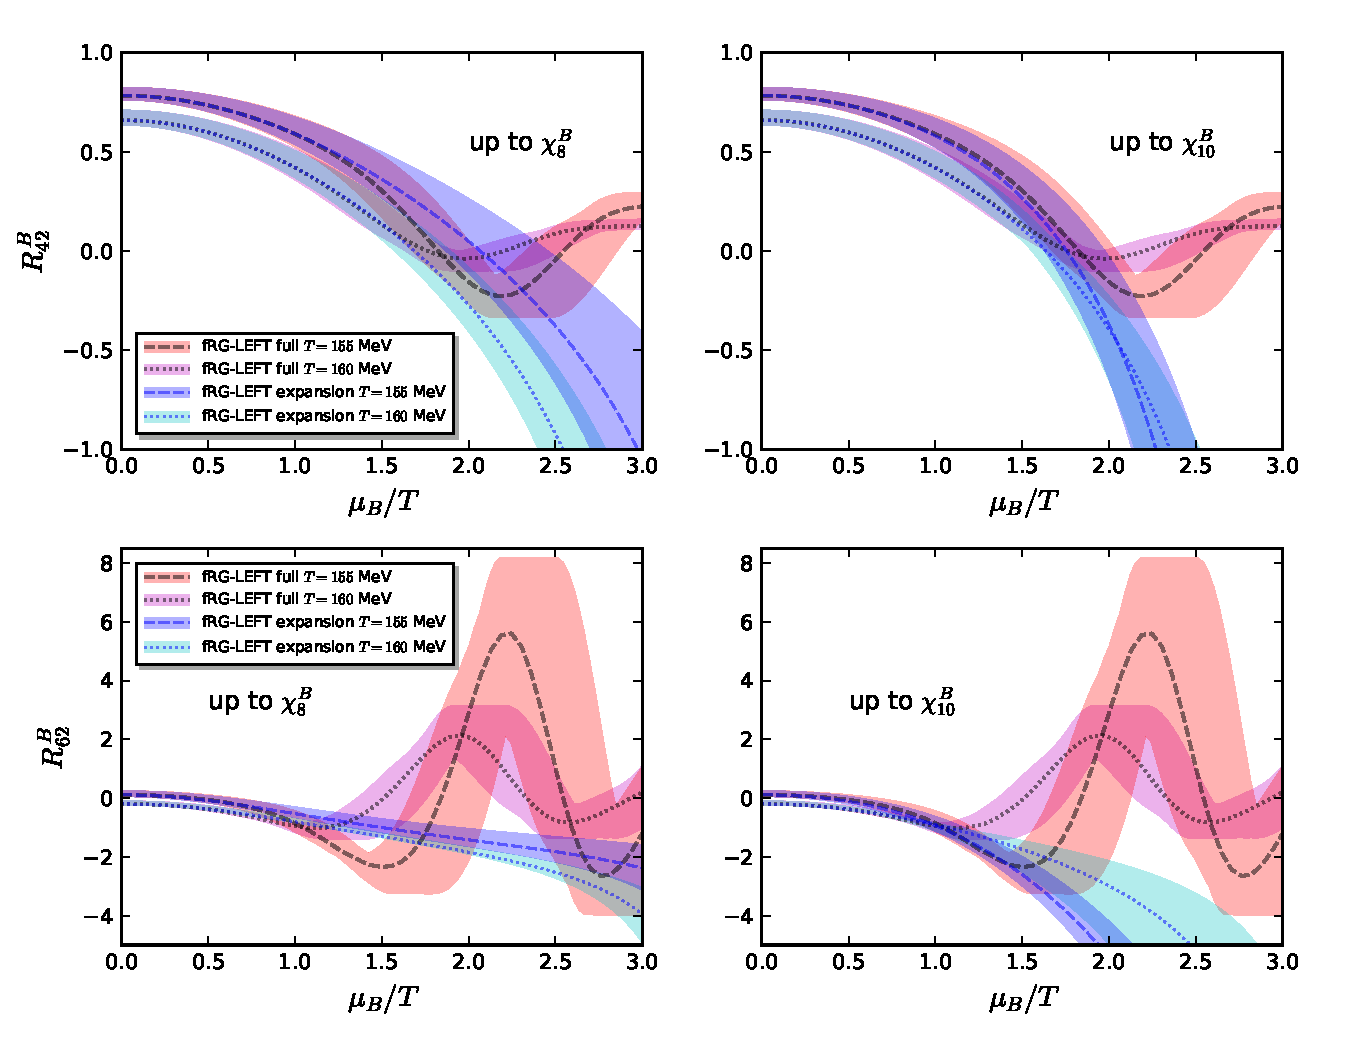
\includegraphics[width=0.9\textwidth]{R42R62expansion-muBoT}
\caption{Comparison between the direct calculation of baryon number fluctuations $R^{B}_{42}$ (upper panels) and $R^{B}_{62}$ (lower panels) via \eq{eq:suscept} at finite $\mu_B$ and the Taylor expansion up to $\chi^B_8(0)$ in \eq{eq:chiBTay} (left panels) and to $\chi^B_{10}(0)$ (right panels). Both calculations are performed within the QCD-assisted LEFT used in the present work. $R^{B}_{42}$, $R^{B}_{62}$ are shown as functions of $\mu_B/T$ with $T=155$ MeV and $T=160$ MeV.}\label{fig:R42R62expansion-muBoT}
\end{figure*}
%%%%%%%%%%%%%%%%%%%%%%%%%%%%%
%

For the evaluation of the reliability regime of the Taylor expansion about vanishing chemical potential we consider the Taylor expansion of the pressure in \Eq{eq:pres} in powers of $\hat{\mu}_{B}\equiv\mu_B/T$ around $\hat{\mu}_{B}=0$. This leads us to 
%
\begin{align}
\frac{p(\mu_B)}{T^4}&=\frac{p(0)}{T^4}+\sum_{i=1}^{\infty}\frac{\chi^B_{2i}(0)}{(2i)!}\,\hat{\mu}_{B}^{2i}\,,\label{eq:cmu}
\end{align}
%
with the expansion coefficients $\chi^B_{2i}(0)=\chi^B_{2i}(\mu_B=0)$, the hyper-order fluctuations of the baryon charge. In \Eq{eq:cmu} we have suppressed the temperature-dependence of all functions for the sake of readability. Truncating the Taylor expansion in \Eq{eq:cmu} at the eighth order, $\hat{\mu}_{B}^{8}$, and employing \eq{eq:suscept}, we obtain the expanded baryon number fluctuations, 
%
\begin{align}
\chi^B_2(\mu_B)\simeq&\chi^B_2(0)+\frac{\chi^B_4(0)}{2!}\hat{\mu}_{B}^{2}+\frac{\chi^B_6(0)}{4!}\hat{\mu}_{B}^{4}+\frac{\chi^B_8(0)}{6!}\hat{\mu}_{B}^{6}\,,\nonumber \\[2ex]
\chi^B_4(\mu_B)\simeq&\chi^B_4(0)+\frac{\chi^B_6(0)}{2!}\hat{\mu}_{B}^{2}+\frac{\chi^B_8(0)}{4!}\hat{\mu}_{B}^{4}\,,\nonumber\\[2ex]
\chi^B_6(\mu_B)\simeq&\chi^B_6(0)+\frac{\chi^B_8(0)}{2!}\hat{\mu}_{B}^{2}\,.\label{eq:chiBTay}
\end{align}
%
In \Fig{fig:R42R62-muBoT} we show the ratios $R^B_{42}=\chi^B_4/\chi^B_2$ and $R^B_{62}=\chi^B_6/\chi^B_2$ based on the Taylor expansion for two fixed temperatures:  $T=155$\,MeV (close to the crossover temperature $T_c$ at $\mu_B=0$) and $T=160$\,MeV (slightly above $T_c$). As an input we use $\chi^B_{2i}(0)$ ($i \!=\! 1,\, 2,\, 3,\, 4$) from the current setup as well as from the lattice (HotQCD collaboration \cite{Bazavov:2020bjn} and Wuppertal-Budapest collaboration \cite{Borsanyi:2018grb}), depicted already in \Fig{fig:R42R62R82-T-muB0}. As expected, the LEFT-results for the $\mu_B$-dependence of $R^{B}_{42}$ and $R^{B}_{62}$ agrees qualitatively with both lattice results. Moreover, it agrees quantitatively with the Wuppertal-Budapest result.   

Since we are not restricted by a sign problem within the fRG approach, the $\chi^B_n(\mu_B)$'s in \Eq{eq:suscept} can also be computed directly for the current QCD-assisted LEFT without resorting to a Taylor expansion. By comparing this to the results of the Taylor expansion, we can study its range of validity. The results are presented in the left panel of \Fig{fig:R42R62expansion-muBoT}, again for $T=155$\,MeV and $T=160$\,MeV and with the Taylor expansion up to eights order in $\hat \mu_B$.


We observe that the result for $R^{B}_{42}$ from the Taylor expansion in \Eq{eq:chiBTay} agrees quantitatively with that from the full calculation for $\mu_B/T\lesssim 1.2$ for $T=155$\,MeV and $\mu_B/T\lesssim 1.5$ for $T=160$\,MeV. Not surprisingly, this reliability regime is reduced significantly for the hyper-order fluctuation $R^{B}_{62}$ to $\mu_B/T\lesssim 1.2$ for $T=160$\,MeV and $\mu_B/T\lesssim 0.8$ for $T=155$\,MeV. 
For larger $\mu_B/T$, the fluctuations show a non-trivial oscillatory behaviour that cannot be captured by a (low-order) Taylor expansion. We emphasise that this is not an artefact of our model, but rather a generic, physical feature of these fluctuation observables. It reflects the increasingly pronounced non-monotonic temperature dependence of $R^{B}_{n2}$ due to long-range correlations in the crossover region, as seen in \Fig{fig:R42R62R82-T-muB0to400}. In particular, $R^{B}_{n2}$ develops distinctive areas around the crossover at larger $\mu_B$ where its value varies significantly, even including sign changes. By following a line of fixed $T$ close to $T_c$ and increasing $\mu_B$ in the phase diagram, these areas are crossed eventually, leading to the oscillatory behaviour seen in \Fig{fig:R42R62expansion-muBoT}. This is also evident in the right plot of \Fig{fig:phasediagram}, where we show the magnitude of $R^{B}_{42}$ in the phase diagram. Since these strong fluctuations only occur at larger $\mu_B$, the resulting characteristic qualitative features cannot be captured by a (low-order) Taylor expansion at $\mu_B=0$; it is bound to fail at the onset of the oscillatory behaviour, i.e.\ around $\mu_B/T \gtrsim 1$. 

It is also interesting to evaluate to what extend a higher-order Taylor expansion can improve its reliability. We therefore include our prediction for $R^B_{10\, 2}$ from \fig{fig:R102-T-muB0}, hence extending the Taylor expansion in \Eq{eq:chiBTay} to the tenth order. The resulting comparison is shown in right panel of \Fig{fig:R42R62expansion-muBoT}. Interestingly, this does not change the compatibility regime for $T=160$\,MeV significantly. In turn, there are significant changes for $T=155$\,MeV. While the deviations for $R_{42}^B$ 
start to grow at roughly the same $\mu_B/T$ as for the eights-order expansion, that is $\mu_B/T\lesssim 1.2$, the result for $R_{42}^B$ stays compatible with the full result for larger values. For $R_{62}^B$ the reliability regime is essentially doubled: it rises from $\mu_B/T\lesssim 0.8$ to $\mu_B/T\lesssim 1.5$. 

The analysis above suggests the following picture: We have a temperature-dependent radius of convergence, 
%
\begin{align}\nonumber 
 T=155\,\textrm{MeV}:\quad &[\mu_B/T]_\textrm{Max}\approx 1.5\,,\\[1ex] T=160\,\textrm{MeV}:\quad &[\mu_B/T]_\textrm{Max}\approx 1.2\,.
\label{eq:RadiusConverge}\end{align}
%
Moreover, the results have already converged for $R_{42}^B,R_{62}^B$ for $T=160$\,MeV as well as for $R^B_{42}$ for $T=155$\,MeV within the eighth order and for $\mu_B/T\lesssim [\mu_B/T]_\textrm{Max}(T)$. In turn, convergence for $R^B_{62}$ for $\mu_B/T\lesssim  [\mu_B/T]_\textrm{Max}$ requires the tenth order Taylor expansion for $T=155$\,MeV. For a discussion of the radius of convergence based on mean-field theory we refer to \cite{Karsch:2010hm}. In general, it is given by the distance to the nearest singularity of the equation of state in the complex $\mu_B/T$ plane. Hence, possible candidates for this singularity are the CEP, the Roberge--Weiss endpoint at imaginary $\mu_B$ \cite{Roberge:1986mm}, or the Yang--Lee edge singularity in the complex plane \cite{Yang:1952be}. Evidently, the distance to the CEP is far larger than the radius estimated here. In turn, the closest endpoint at imaginary chemical potential is at $|\mu_B/T|\leq \pi$. For physical quark masses it is most probably close to $|\mu_B/T|=\pi$. For a discussion within QCD-flows see~\cite{Braun:2009gm}, for lattice results see e.g.~\cite{Philipsen:2014rpa}. Hence, a particularly intriguing option is the Yang--Lee edge singularity, for a discussion see e.g.~\cite{Stephanov:2006dn, Mukherjee:2019eou}. However, while the location of the edge singularity has been determined for critical $O(N)$ theories \cite{Connelly:2020gwa}, it is still unknown for QCD.

This interpretation also implies that the results from the Taylor expansion fail to agree even qualitatively with the correct $\mu_B/T$-dependence for $\mu_B/T_c \gtrsim [\mu_B/T]_\textrm{Max}(T)$, see  \fig{fig:R42R62expansion-muBoT}. Interestingly, $[\mu_B/T]_\textrm{Max}(T)$ seems to grow for smaller temperatures. Whether or not this holds true requires a more systematic study, which will be considered elsewhere. In conclusion, the extrapolation of fluctuations of conserved charged in the vicinity of the chiral crossover within a Taylor expansion loses its predictive power for $\mu_B\gtrsim 200$\,MeV, at least at tenth order.  

%
%%%%%%%%%%%%%%%%%%%%%%%%%%%%%
\begin{figure*}[t]
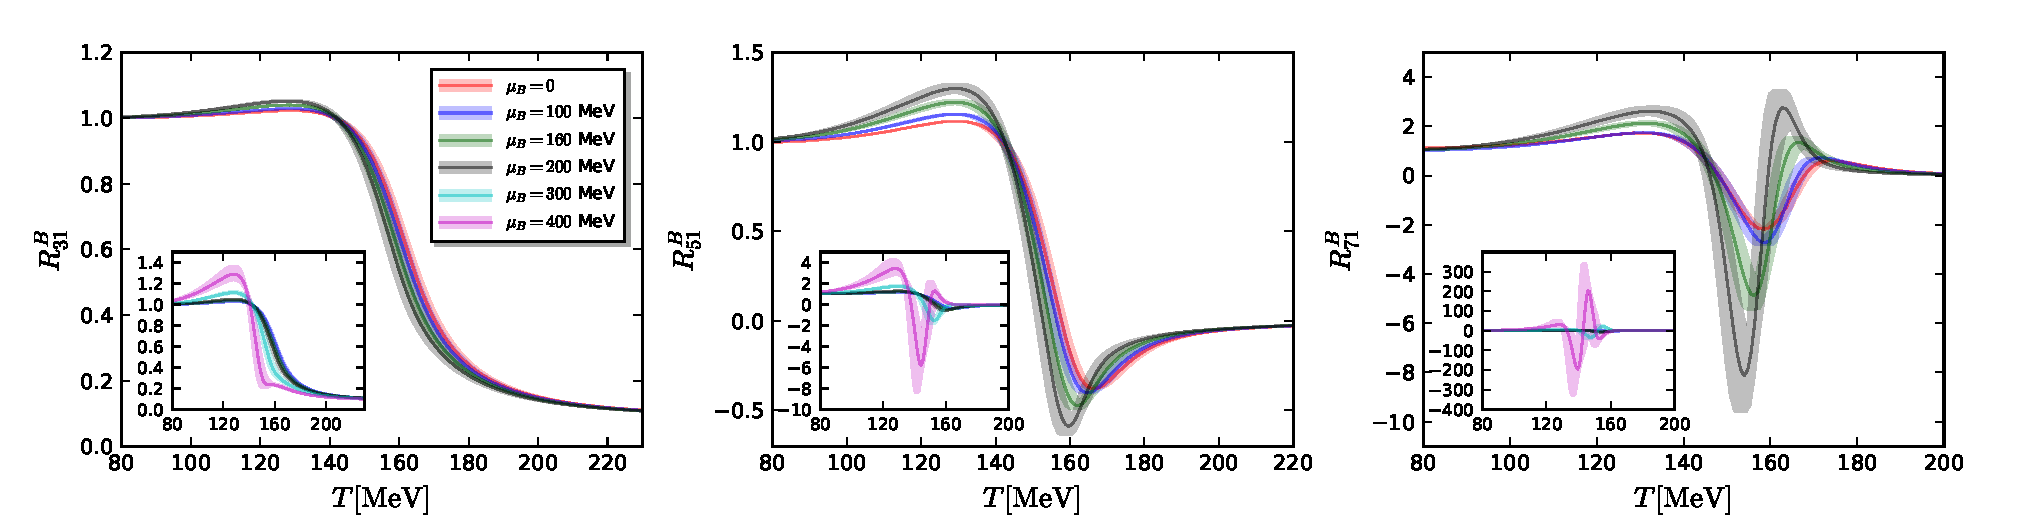
\includegraphics[width=1.\textwidth]{R31R51R71-T-muB0to400}
\caption{$R^{B}_{31}$ (left panel), $R^{B}_{51}$ (middle panel), and $R^{B}_{71}$ (right panel) as functions of the temperature at several values of $\mu_B$. Insets in each plot show their respective zoomed-out view. }\label{fig:R31R51R71-T-muB0to400}
\end{figure*}
%%%%%%%%%%%%%%%%%%%%%%%%%%%%%
%

This raises the important question of whether one can manage to describe the peculiar behaviour of the full result within a resummation of the Taylor series, that may also take into account information from fluctuation data at finite baryon chemical potential. There, also odd fluctuations are non-vanishing. In \fig{fig:R31R51R71-T-muB0to400} we therefore show our temperature-dependence of $R^B_{31}$, $R^B_{51}$, and $R^B_{71}$ for different baryon chemical potentials. A further relevant odd fluctuation observable is $R^B_{32}$, depicted in \fig{fig:R32-T-muB0to400}. Its experimental analogue, the proton number fluctuation $R^p_{32}$ has been already measured in Au+Au central (0-5\%) collisions at STAR, a comparison will be presented and discussed in \sec{sec:CEP}.  

If such a resummation is possible and stable against variations within the present QCD-assisted LEFT, it would be suggestive that the same  resummation formula also works for QCD-data for hyper-fluctuations at vanishing density. Together with work on hyper-fluctuations in an extension of the functional QCD-work in \cite{Fu:2019hdw} this could finally provide a quantitatively reliable extrapolation approach for fluctuation observables in QCD. 
%
%%%%%%%%%%%%%%%%%%%%%%%%%%%%
\begin{figure}[b]
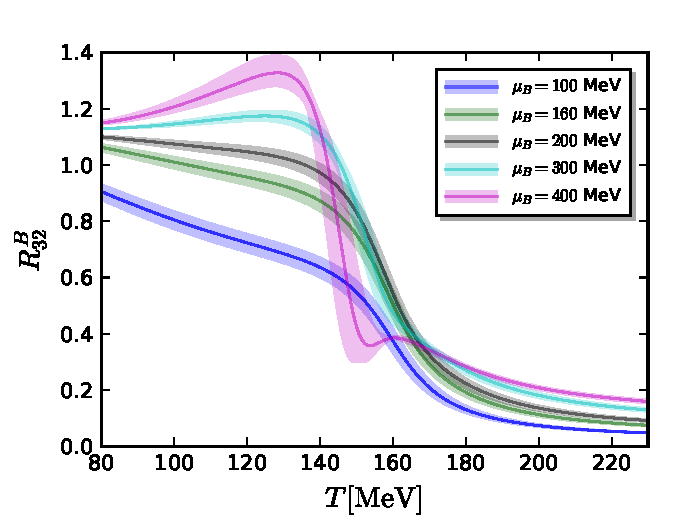
\includegraphics[width=0.45\textwidth]{R32-T-muB0to400}
\caption{Baryon number fluctuation $R^{B}_{32}$ as a function of the temperature at several values of $\mu_B$. }\label{fig:R32-T-muB0to400}
\end{figure}
%%%%%%%%%%%%%%%%%%%%%%%%%%%%%
%


%%%%%%%%%%%%%%%%%%%%%%%%%%%%%%%%%%%%%%%%%%%%%%%%%%%%%%%%%%%%%%%%%

\subsection{Determination of the  freeze-out curve}
\label{subsec:freezeoutCurve}	

%
%%%%%%%%%%%%%%%%%%%%%%%%%%%%%
\begin{figure*}[t]
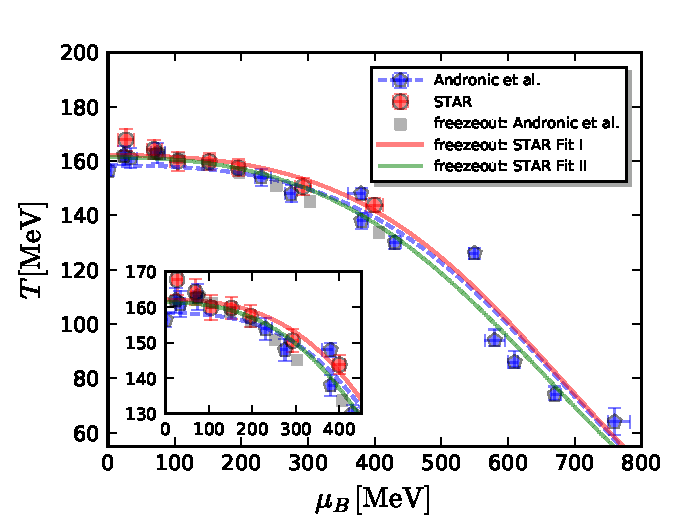
\includegraphics[width=0.42\textwidth]{phasediagram}
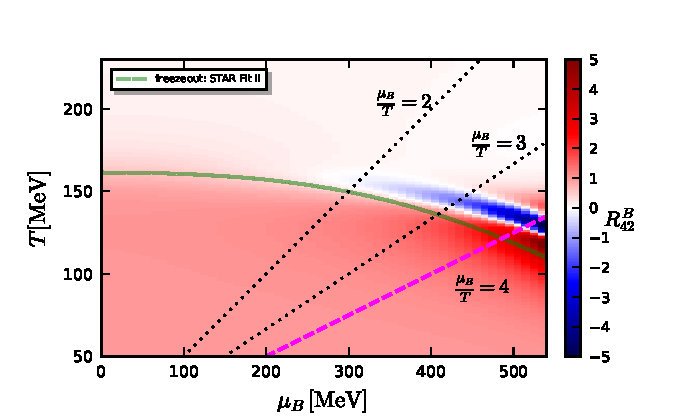
\includegraphics[width=0.55\textwidth]{R42phasediagram}
\caption{Left panel: chemical freeze-out temperature and baryon chemical potential in the $T\!-\!\mu_B$ plane. The blue pentagons and red circles show the freeze-out data from Andronic {\it et al.} \cite{Andronic:2017pug} and STAR experiment \cite{Adamczyk:2017iwn}, respectively. The blue dashed line represents the parametrisation of blue pentagons through \eq{eq:muBCFparatri} and \eq{eq:TCFparatri}. The red solid and green dotted lines show the parametrisation of the STAR data based on all the seven data points, and only the four data points in the middle region ($100\,\mathrm{MeV}\lesssim\mu_B\lesssim 300\,\mathrm{MeV}$), respectively. The grey squares are obtained by interpolating the blue pentagons. The inlay zooms in the low-$\mu_B$ region. \\ 
Right panel: Baryon number fluctuations $R^{B}_{42}$ in the $T\!-\!\mu_B$ plane. The freeze-out curve is the STAR Fit II. The dashed line at $\mu_B/T=4$ constitutes the reliability bound of the computations in \cite{Fu:2019hdw} based on the potential emergence of new degrees of freedom discussed in \cite{Fu:2019hdw, Braun:2019aow, Fischer:2018sdj}. The dashed lines at $\mu_B/T=2,3$ are reliability estimates of lattice results as well as old ones from functional approaches, see also \Fig{fig:QCD-scalematching}.}\label{fig:phasediagram}
\end{figure*}
%%%%%%%%%%%%%%%%%%%%%%%%%%%%%
%

The quantitatively successful benchmark tests analysed in \sec{subsec:hyper-order0}, and the evaluation of baryon number fluctuations at finite chemical potential in \sec{subsec:hyper-ordermuB} allow us to discuss our main goal: the comparison of theoretical predictions on the baryon number fluctuations with experimental measurements. 

A direct comparison between theory and experiment is a very  challenging task. This is due to the fact that experimental data are affected by many factors. First, this concerns the acceptance of the detector such as the transverse momentum $p_T$ range, rapidity window and the centrality dependence, e.g.\ \cite{Adamczyk:2013dal,Luo:2015ewa,Bzdak:2016sxg, He:2017zpg,Adam:2020unf,Nonaka:2020crv,Pandav:2020uzx}, see \cite{Luo:2017faz,Adamczyk:2017iwn} for more details. Second, the physics setup used in theory and experiment may differ by the presence of volume fluctuations, e.g.\  \cite{Luo:2013bmi,Chatterjee:2019fey,Chatterjee:2020nnn}, finite volume effects on the location of the chiral phase boundary, e.g.\ \cite{Braun:2010vd, Braun:2011iz, Tripolt:2013zfa, Almasi:2016zqf, Klein:2017shl, Li:2017zny, Liu:2020elq, Wan:2020vaj}, the question of global baryon number conservation, e.g.\  \cite{He:2016uei,Braun-Munzinger:2016yjz,Vovchenko:2020tsr}, the inclusion of resonance decays, e.g.\  \cite{Nahrgang:2014fza,Zhang:2019lqz}, and others. 

All these different effects and experimental restrictions give rise to  non-critical contributions to fluctuation observables in experiments, and pinning down their contributions plays a pivotal role in identifying the critical signals in the BES experiment. Additionally, due to critical slowing down, non-equilibrium effects become important in the vicinity of the CEP \cite{Berdnikov:1999ph}, which necessitates a theoretical description of the dynamics of critical fluctuations. For more details about recent progress on the dynamics of critical fluctuations in QCD, see \cite{Bluhm:2020mpc} and references therein. We emphasise, however, that the present results of QCD-assisted LEFT model are well outside the critical region. Therefore they are not subject to critical scaling in the vicinity of the CEP. 

In this work we will not take into account the non-critical and dynamical effects discussed above. Instead, we assume that the measured cumulants of the net-proton multiplicity distribution at a given collision energy are in one-to-one correspondence to the calculated fluctuations in \Eq{eq:suscept} with single values for $T$ and $\mu_B$ (with other collision parameters e.g., the centrality and rapidity range fixed). Then, it is suggestive to identify the values of $T$ and $\mu_B$ with the ones when the chemical freeze-out occurs, viz. $T_{_{\textrm{CF}}}$ and ${\mu_B}_{_{\textrm{CF}}}$. Such an approach for the comparison is usually employed in fluctuation studies of equilibrium QCD matter within functional methods or lattice simulations, see e.g.\ \cite{Fu:2015amv, Fu:2016tey, Almasi:2017bhq, Isserstedt:2019pgx, Bazavov:2020bjn}.

We adopt the freeze-out temperatures and baryon chemical potentials from \cite{Andronic:2017pug} and from the STAR experiment \cite{Adamczyk:2017iwn}, which are shown in the left panel of \Fig{fig:phasediagram} by the blue pentagons and red circles, respectively. They are both obtained from the analysis of hadron yields in the statistical hadron resonance gas model, see the  aforementioned references for more details. The freeze-out data in \cite{Andronic:2017pug} has also been parametrised as functions of the collision energy as follows 
%
\begin{subequations}\label{eq:freeze-outFit}
%
\begin{align}
{\mu_B}_{_{\textrm{CF}}}&=\frac{a}{1+0.288\sqrt{s_{\mathrm{NN}}}},\label{eq:muBCFparatri}
\end{align}
%
with $a=1307.5$ MeV, and
%
\begin{align}
T_{_{\textrm{CF}}}&=\frac{T^{(0)}_{_{\textrm{CF}}}}{1+\exp\big(2.60-\ln(\sqrt{s_{\mathrm{NN}}})/0.45\big)},\label{eq:TCFparatri}
\end{align}
%
\end{subequations}
%
with $T^{(0)}_{_{\textrm{CF}}}=158.4$ MeV. This parametrisation is depicted with the blue dashed line in the left panel of \Fig{fig:phasediagram}. We use the same parametrisation functions in \Eq{eq:freeze-outFit} to fit the freeze-out data in STAR experiment, i.e., the red circle points. For this fit we invoke two procedures, called STAR Fit I \& II in the following: \\[-2ex]

For the first one, STAR Fit I, we simply take all 7 data points. The corresponding freeze-out curve is depicted by the red solid line in the left panel of \fig{fig:phasediagram}. 

%
%%%%%%%%%%%%%%%%%%%%%%%%%%%%%
\begin{figure*}[t]
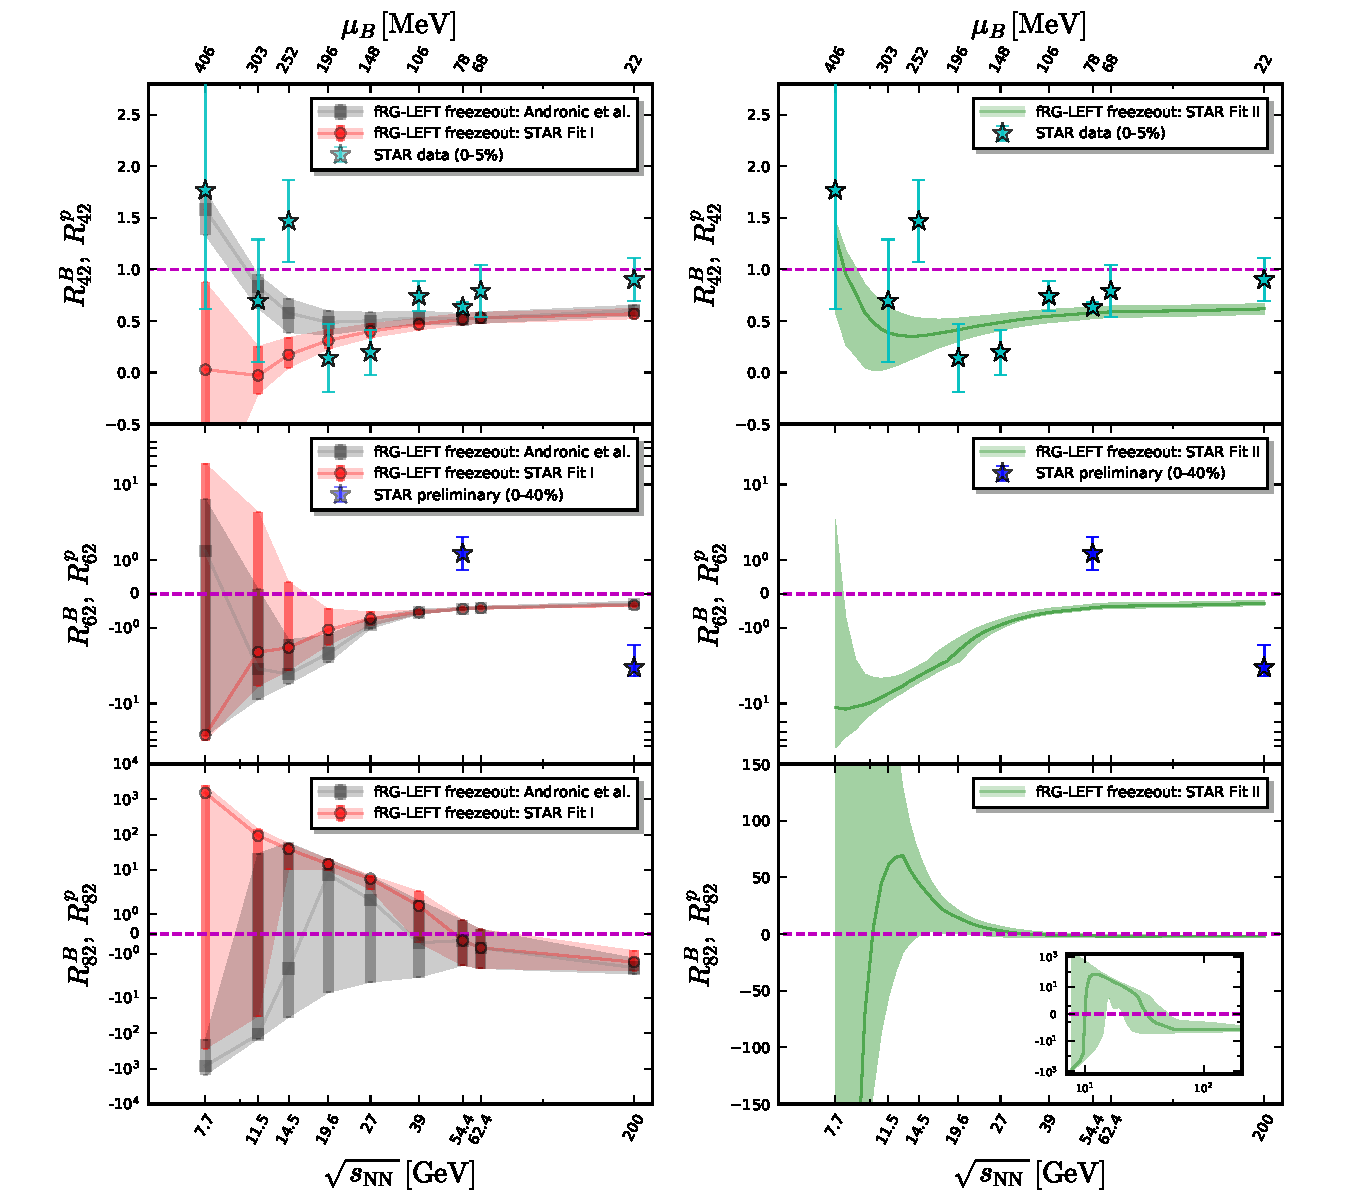
\includegraphics[width=0.9\textwidth]{Rm2-sqrtS}
\caption{QCD-assisted LEFT (fRG-LEFT): Baryon number fluctuations $R^{B}_{42}$ (top), $R^{B}_{62}$ (middle), and $R^{B}_{82}$ (bottom) as functions of the collision energy. 
Left panels: the freeze-out points are those from Andronic {\it et al.} \cite{Andronic:2017pug} (grey) and the STAR experiment \cite{Adamczyk:2017iwn} (red).
Right panels: The freeze-out curve, STAR Fit II, is obtained from the freeze-out parameters of the STAR experiment \cite{Adamczyk:2017iwn}. 
The theoretical error bands show a highly correlated error, and should be interpreted as a family of curves with the same qualitative behaviour as the central curve. For more explanations see \sec{subsec:freezeoutCurve} with \fig{fig:phasediagram}. 
\newline
STAR data: $R^{p}_{42}$ (top) is the kurtosis of the net-proton distributions measured in Au+Au central (0-5\%) collisions \cite{Adam:2020unf}. $R^{p}_{62}$ (middle) is the preliminary result on the six-order cumulant of the net-proton distribution at $\sqrt{s_{\mathrm{NN}}}$=200 GeV and 54.4 GeV with centrality 0-40\% \cite{Nonaka:2020crv,Pandav:2020uzx}. 
}\label{fig:Rm2-sqrtS}\vspace{-0.5cm}
\end{figure*}
%%%%%%%%%%%%%%%%%%%%%%%%%%%%%
%
For the construction of the second one, STAR Fit II, we shall argue that some of the data points are potentially flawed, or rather await a physics explanation, and should be dropped accordingly in a fit based on \eq{eq:freeze-outFit}. Accordingly, we drop the first two data points at small chemical potential as well as the last one at the largest available chemical potential $\mu_B\sim 400$. From general considerations we do not expect the freeze-out curve to rise with increasing chemical potential. Moreover, the physically motivated fit formula does not describe sign-changes of the curvature of the freeze-out curve. For a respective discussion and possible explanation for the only apparent rise see \cite{Bluhm:2020rha}. The last data point is also not well-described by the fitting procedure described here. This may indicate the onset of a regime with different physics/phases. In this case, \Eq{eq:freeze-outFit} would not be an appropriate fit function. It may also indicate the onset of a regime of rapidly worsening systematics. In this case more points are needed in this regime.  

The freeze-out line of STAR Fit II is depicted by the green dotted line in the left panel of \fig{fig:phasediagram}. In comparison to STAR Fit I, STAR Fit II is located at slightly lower temperatures, which is more pronounced when $\mu_B\gtrsim 200$\,MeV. In the right panel of \Fig{fig:phasediagram}, we show the baryon number fluctuation $R^{B}_{42}$ in the $T\!-\!\mu_B$ plane. It can be observed that a narrow blue band, indicating the regime of negative $R^{B}_{42}$, develops around the crossover starting at $\mu_B\sim 250$ MeV. The freeze-out curve STAR Fit II is approaching towards the boundary of the blue region firstly at small $\mu_B$, and then deviates a bit from it at large $\mu_B$. We emphasise that the large chemical potential region, and in particular  asymptotically large $\mu_B\gtrsim 500$ MeV, is beyond of the reliability bound of the current computation, $\mu_B/T=4$, see \Fig{fig:QCD-scalematching}. For a detailed discussion see \sec{subsec:scale}.



%%%%%%%%%%%%%%%%%%%%%%%%%%%%%%%%%%%%%%%%%%%%%%%%%%%%%%%%%%%%%%%%

\subsection{Hyper-order baryon number fluctuations on the  freeze-out curve}
\label{subsec:freezout}	

The determination of the freeze-out curve completes our setup, which enables us to compute hyper-order baryon number fluctuations $R_{nm}^B$ along the freeze-out line within the QCD-assisted LEFT. These results are then used to compare with the experimental measurements of cumulants $R_{nm}^p$ of the net-proton distribution from STAR experiment. 

Before we discuss the numerical results, we also emphasise once more, that it follows from the analysis of \sec{subsec:hyper-ordermuB}, that the simple extrapolation with the Taylor expansion about $\mu_B=0$ lacks predictive power for $\mu_B\gtrsim 250$\,MeV, that is $\sqrt{s_{\rm NN}}\lesssim 15$\,GeV, see \Eq{eq:RadiusConverge}. Moreover, it even lacks predictive power for the qualitative behaviour. 

In the left panel of \Fig{fig:Rm2-sqrtS} we show the $\sqrt{s_{\rm NN}}$- or chemical potential dependence of the baryon number fluctuations $R^{B}_{42}$, $R^{B}_{62}$, and $R^{B}_{82}$ for the freeze-out lines from Andronic {\it et al.} \cite{Andronic:2017pug} and STAR Fit I. The freeze-out line from Andronic {\it et al.} is obtained from an interpolation of the freeze-out data, the grey squares in \fig{fig:phasediagram}. 

In the right panel of \Fig{fig:Rm2-sqrtS} we show the same observables for the freeze-out line of STAR Fit II. As discussed in \sec{subsec:freezeoutCurve}, we have singled out the results for this freeze-out curve as the best-informed computation. 

In both panels of \fig{fig:Rm2-sqrtS} we also show the experimental measurement of cumulants of the net-proton distributions in the beam energy scan experiments from the STAR collaboration. The fourth-order fluctuations, $R^{p}_{42}$, of the net-proton multiplicity distributions are measured in Au+Au collisions with centrality 0-5\%, transverse momentum range $0.4< p_T\,(\mathrm{GeV}/c)\,<2.0$, and rapidity $|y|<0.5$, cf. \cite{Adam:2020unf} for more details. Moreover, preliminary results for the sixth-order cumulant of the net-proton distribution, $R^{p}_{62}$, are also presented in the middle plot of \Fig{fig:Rm2-sqrtS}, which are obtained at two values of the collision energy, i.e., $\sqrt{s_{NN}}$=200 GeV and 54.4 GeV with centrality 0-40\% \cite{Nonaka:2020crv,Pandav:2020uzx}. 

The theoretical results for the fourth-order fluctuations $R^B_{42}$ from the present QCD-assisted LEFT for all freeze-out curves considered are compatible with the respective experimental measurement of the $\kappa\sigma^{2}$ of net-proton distributions in 0-5\% central Au+Au collisions. 
In particular, the theoretical  results feature a  non-monotonic $\sqrt{s_{\rm NN}}$-dependence: $R^B_{42}$ first decreases with increasing beam energy and then increases. The details of this behaviour, in particular how pronounced it is, is highly sensitive to the precise location of the freeze-out. For example, the increase at small $\sqrt{s_{\rm NN}}$ is larger for smaller freeze-out temperatures. Thus, the weak increase for STAR Fit 1 originates in the slightly larger freeze-out temperature of this freeze-out fit. 
This shows that even small variations in the freeze-out temperature have a substantial effect on the fluctuations in this regime. The underlying reason is that the freeze-out happens in or close to the crossover region, where the fluctuations vary significantly, see \Fig{fig:R42R62R82-T-muB0to400}. Importantly, this regime cannot be accessed within the extrapolation of the Taylor expansion at least within the current order.

This entails that extrapolations based on a Taylor expansion are bound to fail to describe the data in this regime reliably. Consequently this calls for qualitatively improved direct theoretical computations at small bean-energies. This is work in progress and we hope to report on the respective results soon. 

Our results for the hyper-order fluctuations $R^B_{62}$ and $R^B_{82}$ are shown in the middle and bottom panel of \Fig{fig:Rm2-sqrtS}. For small chemical potentials or large collision energies both fluctuation observables are negative. Moreover, $R^B_{62}$ decreases with decreasing $\sqrt{s_\mathrm{NN}}$, while $R^B_{82}$ increases. The occurrence of non-monotonicities of $R^B_{62}$ and $R^B_{82}$ at lower beam energies cannot be shown within the accuracy limits of the current study.

For $\sqrt{s_\mathrm{NN}}$=200 GeV and 54.4 GeV we can compare our results for $R^{B}_{62}$ to preliminary STAR data within 0-40\% centrality \cite{Nonaka:2020crv,Pandav:2020uzx}. At the highest beam energy, $\sqrt{s_\mathrm{NN}}$=200 GeV, we agree qualitatively in that $R^{B}_{62}$ is negative. However, the STAR result at 54.4 GeV for 0-40\% centrality shows positive values and large deviation from our model result. We need to point out that a direct comparison is difficult at this point and conclusion would be premature. In our opinion these large deviations at small chemical potential points at a lack of a complete physics interpretation of the experimental data. 

Another interesting property of the current LEFT setting is that the non-monotonic behaviour of our results for $R^{B}_{n2}$ at large $\mu_{B}$ in \Fig{fig:Rm2-sqrtS} does not arise from critical physics: in the LEFT used here, the CEP is at significantly larger $\mu_B\gtrsim 700$\,MeV. Moreover, it is well established that the critical region is only very small. It is already small within mean-field approximations of low-energy effective theories, and additionally shrinks considerably if quantum, thermal and density equilibrium fluctuations are taken into account, see \cite{Schaefer:2006ds}. Moreover, this does not change if transport processes are taken into account, see \cite{Bluhm:2018qkf}. 

In the present LEFT the increasing trend at large $\mu_{B}$ region originates from two effects: First, fluctuations are enhanced since the chiral crossover becomes sharper with increasing $\mu_B$. This leads to a stronger non-monotonic behaviour of $R^{B}_{42}$ as a function of $T$, see \Fig{fig:R42R62R82-T-muB0to400}. This sharpening is also present in the vicinity of a CEP. Second, the freeze-out temperature is shifted away from the pseudo-critical temperature towards small beam-energies, thereby probing different regimes of the cumulants. However, it should be noted that the uncertainty of our results increases significantly in the low energy region. These uncertainties include an estimate for the systematic error of the QCD-assisted LEFT-approach. This systematic error stems from the uncertainty in the matching of the in-medium scales of the LEFT and QCD, encoded in the coefficients $c_{_{T}}$ and $c_{\mu}$ in \Eq{eq:rescale}. Moreover, for larger chemical potential the current LEFT lacks the back-reaction of the $\mu_B$-dependence of the glue-dynamics. While inherently small, it might still play a r$\hat{\textrm{o}}$le. 

%%%%%%%%%%%%%%%%%%%%%%%%%%%%%%%%%%%%%%%%%%%%%%%%%%%%%%%%%%%%%%%%%%%%%

\subsection{Search for the CEP} \label{sec:CEP}

%
%%%%%%%%%%%%%%%%%%%%%%%%%%%%
\begin{figure*}[t]
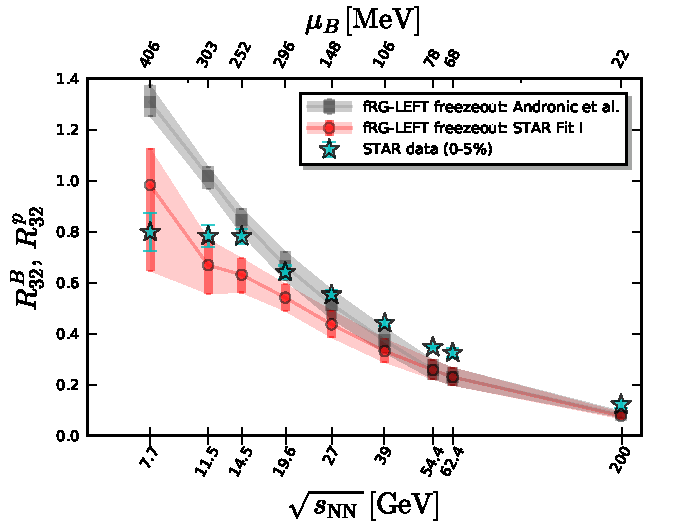
\includegraphics[width=0.48\textwidth]{R32-sqrtS-other}
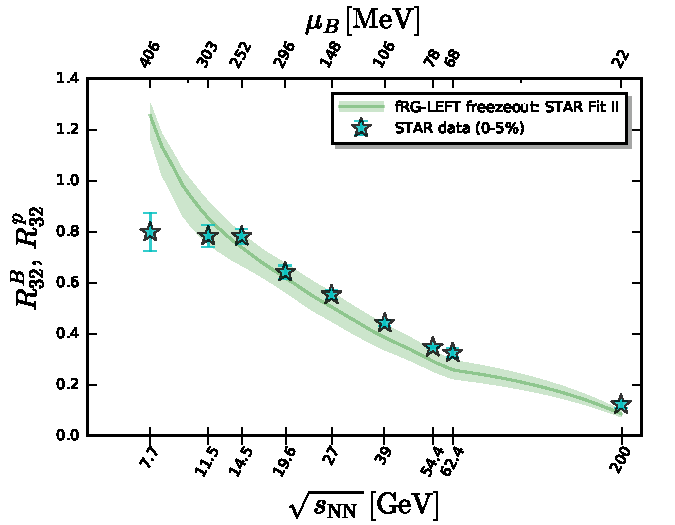
\includegraphics[width=0.48\textwidth]{R32-sqrtS}
\caption{Baryon number fluctuation $R^{B}_{32}$ as a function of the collision energy in comparison to STAR-data for $R^{p}_{32}$ (0-5\%) centrality. 
Left panel: the freeze-out points are those from Andronic {\it et al.} \cite{Andronic:2017pug} (grey) and the STAR experiment \cite{Adamczyk:2017iwn} (red).
Right panel: The freeze-out curve, STAR Fit II, is obtained from the freeze-out parameters of the STAR experiment \cite{Adamczyk:2017iwn}. 
The theoretical error bands show a highly correlated error, and should be interpreted as a family of curves with the same qualitative behaviour as the central curve. For more explanations see \sec{subsec:freezeoutCurve} with \fig{fig:phasediagram}. }\label{fig:R32-sqrtS}
\end{figure*}
%%%%%%%%%%%%%%%%%%%%%%%%%%%%%
%

%
%%%%%%%%%%%%%%%%%%%%%%%%%%%%
\begin{figure}[t]
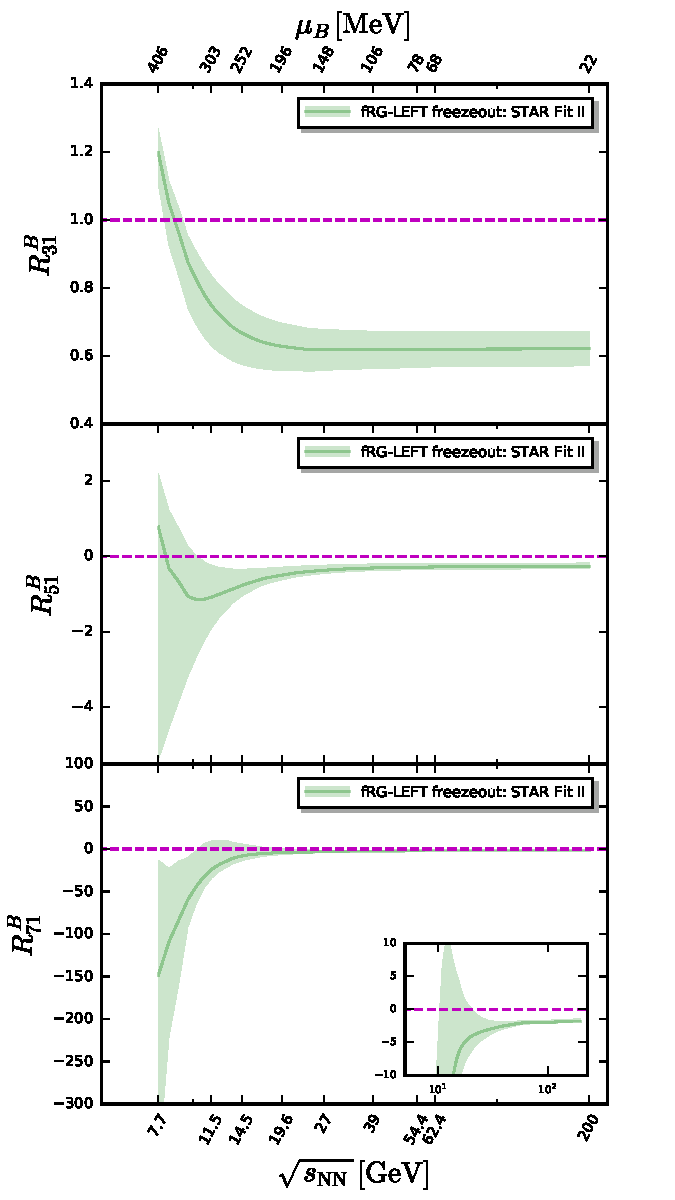
\includegraphics[width=0.45\textwidth]{Rm1-sqrtS}
\caption{Baryon number fluctuations $R^{B}_{31}$ (top), $R^{B}_{51}$ (middle), and $R^{B}_{71}$ (bottom) as functions of the collision energy. 
The freeze-out curve, STAR Fit II, is obtained from the freeze-out parameters of the STAR experiment \cite{Adamczyk:2017iwn}. 
The theoretical error bands show a highly correlated error, and should be interpreted as a family of curves with the same qualitative behaviour as the central curve. For more explanations see \sec{subsec:freezeoutCurve} with \fig{fig:phasediagram}. }\label{fig:Rm1-sqrtS}
\end{figure}
%%%%%%%%%%%%%%%%%%%%%%%%%%%%%
%
The analysis in the previous sections entails that in the present QCD-assisted LEFT the non-monotonic behaviour of  baryon-number fluctuations is triggered by the sharpening of the chiral crossover. This is highly non-trivial, since it is evident, e.g., from \Fig{fig:R42R62R82-T-muB0to400} that neither a system only in the hadronic- nor only in the QGP phase could produce the beam-energy dependencies shown in  \fig{fig:Rm2-sqrtS}. 

In conclusion, the agreement of $R^B_{42}$, computed in the QCD-assisted LEFT and the measured beam-energy dependence of $R^p_{42}$ shows, that the latter could be a signature for the presence of a sharpening crossover between these two phases. Whether or not it also signals the onset of the critical region will be subject of a future improved study. In the context of this latter study we also emphasise that the non-universal properties of the LEFT such as the existence and location of the CEP may not quantitatively agree with QCD as the latter regime lies outside the LEFT-regime with quantitative reliability. Still, the present LEFT probably has the same qualitative non-universal properties at large chemical potential, and it certainly has the same universal ones. 

A non-monotonic energy dependence for the fluctuations is a highly relevant experimental observation, since this behaviour has been proposed as an experimental signature of a CEP \cite{Stephanov:1999zu, Stephanov:2011pb}. The present analysis based on QCD-assisted LEFT model demonstrates that the non-monotonic behaviour of fluctuations can serve as a \textit{indication} of a CEP, but is not necessarily a smoking gun signature for it. The latter requires the extraction of critical scaling, or similar definite signatures such as the detection of a first order regime for large $\mu_B$, etc.\,. 

Still, the non-monotonic behaviour observed in both theory and experiments is a clear \textit{signature} for interesting strongly correlated physics, whose uncovering requires joint and intensified effort of both, theory and experiment. Of course, whether or not these properties carry over completely to QCD remains to be seen. 

Note also that the non-monotonic regime is far away from that covered by a simple extrapolation of the Taylor expansion at $\mu_B=0$. It might be covered by a resummation of the latter, which can already be investigated within the present QCD-assisted LEFT. Constraints on such a resummation should also make use of odd hyper-order fluctuations at finite chemical potential, that are readily computed in the present setup: \\[-1ex] 

A prominent and relevant example is $R_{32}$, already measured in the STAR experiment. In \fig{fig:R32-sqrtS} we show our predictions for $R^B_{32}$ computed in the current QCD-assisted LEFT on the different freeze-out curves defined in \sec{subsec:freezeoutCurve}, see in particular \fig{fig:phasediagram}. In this section it also has been argued, that our best-informed freeze-out curve is given by STAR Fit II. The respective results are shown in the right panel of \fig{fig:R32-sqrtS} in comparison with the STAR data for $R^p_{32}$ (0-5\% centrality). Indeed, these results show the best compatibility with the experimental data. Moreover, within the respective systematic and statistical errors the theoretical results with the freeze-out curve STAR Fit II and the experimental data agree down to collision energies of $\sqrt{s_\mathrm{NN}}\approx$ 14.5\, GeV or $\mu_B\approx 250$\,MeV. 

Interestingly, below $\sqrt{s_\mathrm{NN}}\approx$ 14.5\,GeV the experimental data show a plateau, which is not present in the theoretical prediction. While this is in the large chemical potential regime, in which the LEFT gradually looses its predictive power, also the respective functional first principles QCD computation in \cite{Fischer:2018sdj, Fu:2019hdw, Gao:2020qsj, Gao:2020fbl}, based on a grand potential, do not show any sign of new physics in this regime. This suggests that for  $\sqrt{s_\mathrm{NN}}\lesssim$ 14.5\, GeV at least one of the implicit assumptions underlying the  identification of $R^B_{nm}$ with $R^p_{nm}$ within a grand canonical ensemble with variable baryon charge (density) for given beam energies breaks down. As discussed before, this asks for a re-assessment of the identification of baryon and proton number fluctuations, finite volume effects and finite volume fluctuations, the determination of the freeze-out curve for smaller collision energies, the evaluation of non-equilibrium effects such as transport, and finally the use of the grand potential in the theory computations. While highly relevant and interesting, this goes far beyond the scope of the present work and we defer any further investigation to future work. 

The above example of $R_{32}$ demonstrates very impressively, that the odd (hyper-order) fluctuation observables encode highly relevant physics information which may be difficult or even impossible to extract from the even orders. As a first step in this direction, finally aiming at a resummation of the $\mu_B$-expansion that allows us to go beyond the validity regime of the Taylor expansion, we also have computed the fluctuation observables $R_{31}, R_{51}, R_{71}$ on the freeze-out curve STAR Fit II in \fig{fig:Rm1-sqrtS}. An experimental confirmation of the respective predictions at least for the lower orders would be highly desirable. 

The discussion in this section leaves us with the highly exciting possibility of unravelling the location and properties of a potential CEP within a combined experiment-theory analysis: First principle QCD at finite density should provide us with a prediction for the location of the CEP in terms of hyper-order fluctuations,  $\textrm{Loc}_\textrm{\tiny{CEP}}(R_{nm})$. This would allow us to use the experimental data on hyper-order fluctuation observables $R_{nm}^p$ as input. We emphasise that this prediction does not necessitate the observation of critical behaviour in the $R_{nm}$, but utilises the details of the non-monotonicity of the $R_{nm}$. 

In summary, such an analysis does explicitly not rely on the \textit{universal} property of critical scaling measured in the $R_{nm}$. Indeed, it uses the \textit{non-universal} properties of the $R_{nm}$ to predict the \textit{non-universal} location of the CEP, and hence is far more robust. We hope to report on this matter in the near future. 

%%%%%%%%%%%%%%%%%%%%%%%%%%%%%%%%%%%%%%%%%%%%%%%%%%%%%%%%%%%

\section{Conclusions}
\label{sec:summary}

In this work we have computed baryon number fluctuations up to tenth order with a QCD-assisted low-energy effective theory. This LEFT incorporates quantum, thermal and density fluctuations from momentum scales less than 700\,MeV within the functional renormalisation group approach, and is embedded in QCD, for details see \sec{sec:FRG}. The quantitative predictivity has been benchmarked with a comparison of baryon number fluctuations at $\mu_B=0$ up to the eighth order from the lattice, see \sec{subsec:hyper-order0}. Our results are in quantitative agreement with that from the Wuppertal-Budapest collaboration, and are compatible with that of the HotQCD collaboration, as shown in \fig{fig:R42R62R82-T-muB0}. 

Our direct computation at finite $\mu_B$, presented in \sec{subsec:hyper-ordermuB}, has allowed us to assess the range of validity of the Taylor expansion of the free energy of QCD around $\mu_B = 0$. Such an expansion is commonly used to extrapolate lattice results to finite density. We have shown that the expansion up to tenth order in $\mu_B/T$ is only valid for $\mu_B/T \lesssim 1.5$ in the chiral crossover regime, see \fig{fig:R42R62expansion-muBoT}. Beyond this range, the Taylor expansion, at least to this order, fails to even capture the qualitative behaviour of the fourth- and sixth-order baryon number fluctuations. Thus, results for fluctuations at the freeze-out curve based on a Taylor expansion around $\mu_B=0$ should be interpreted with great caution for $\mu_B/T \gtrsim 1.5$, as relevant physical effects might not be captured by this extrapolation.

The main goal of the current work was the computation of baryon number fluctuations and in particular hyper-order fluctuations along the freeze-out curve at collision energies $\sqrt{s}\gtrsim 7.7$\,GeV. The respective results are discussed in \sec{subsec:freezout}. They have been compared to experimental data of net-proton number cumulants from STAR for different estimates for the freeze-out curve, see \fig{fig:Rm2-sqrtS}. 
Our result for the kurtosis, $R^B_{42}$, is in good agreement with the experimental data for collision energies $\sqrt{s}\gtrsim 7.7$\,GeV. In particular the increasing trend at lower beam energies $\sqrt{s}\lesssim 19.6$\,GeV is captured well. This non-monotonicity is also present in the hyper-order fluctuations $R^B_{62}, R^B_{82}$. We also note that a comprehensive comparison for the higher order cumulants is not possible due to the lack of experimental data. Accordingly, our results in \fig{fig:Rm2-sqrtS} are predictions that await experimental verification. 

We have also investigated the twofold origin of the non-monotonicity for $\sqrt{s}\lesssim 19.6$\,GeV in the present LEFT: First, for increasing chemical potential the chiral crossover gets sharper. Secondly, for smaller beam energies the freeze-out temperature may move away from the pseudo-critical temperatures. In the current setup both phenomena happen far away from a potential critical end point in the LEFT located at $\sqrt{s}_\textrm{CEP} \lesssim 3$\,GeV. The latter regime is also safely outside the reliability regime of the current setup, which gradually looses reliability for $\sqrt{s}\lesssim 27$\,GeV. However, its qualitative features may well be present in QCD. The current LEFT-results and its upgrades towards first principle QCD can be compared with the future experimental results of the high statistic data taken from the second phase of RHIC beam energy scan (BES-II, 2019-2021). From the year of 2018 to 2020, the STAR experiment has collected high statistics data of Au+Au collisions at $\sqrt{s_{\mathrm{NN}}}$ = 9.2, 11.5, 14.6, 19.6 and 27 GeV in the collider mode, and $\sqrt{s_{\mathrm{NN}}}$ = 3.0 -- 7.7 GeV in the fixed target mode. These data give us access to the QCD phase structure for baryon chemical potential up to $\mu_{B}$ $\approx$ 720 MeV. 

Related further steps in a comprehensive understanding of the physics of fluctuations in a heavy ion collision has been undertaken in \sec{sec:CEP}, where we have presented results for odd fluctuations observables $R^B_{31},  R^B_{51}, R^B_{71}$ as well as $R^B_{32}$. While the former observables have not been measured yet, $R^B_{32}$ agrees quantitatively within the systematic and statistical error with the STAR measurement for $R^p_{32}$ for collision energies $\sqrt{s_\mathrm{NN}}\gtrsim$ 14.5\, GeV. For smaller energies, the experimental data show a plateau, the may indicate the loss of one or several of the underlying assumption in the identification of theoretical equilibrium computations of baryon number fluctuations $R^B_{nm}$ in a grand canonical ensemble with the experimental results for proton number fluctuations on the freeze-out curve. 

In summary, the non-monotonicities of hyper-order fluctuations, observed both in experiment and theory, are important  \textit{signatures} for interesting physics in the border regime between quark-gluon plasma and the hadron phase. This of course can include a potential CEP, and in any case deserves further investigation from both experiment and theory. In particular, we envisage that experimental data of fluctuation observables and their dependence on collision energy allow us to constrain the onset regime of this strongly correlated physics/CEP. Importantly, such a prediction does not rely on the observation of critical scaling in the hyper-order fluctuations, but is far more robust, for more details see  \sec{sec:CEP}. We hope to report on this in the near future. 




%%%%%%%%%%%%%%%%%%%%%%%%%%%%%%%%%%%%%%%%%%%%%%%%%%%%%%%%%%%

\begin{acknowledgments}
%
We thank Jens Braun, Rob Pisarski, Bernd-Jochen Schaefer and Nu Xu for discussions. The work was supported by the National Key Research and Development Program of China (Grant No. 2020YFE0202002 and 2018YFE0205201) and the National Natural Science Foundation of China under (Grant No. 11775041, 11828501, 11890711 and 11861131009). The work is also supported by EMMI, and the BMBF grant 05P18VHFCA. It is part of and supported by the DFG Collaborative Research Centre SFB 1225 (ISOQUANT) and the DFG under Germany’s Excellence Strategy EXC - 2181/1 - 390900948 (the Heidelberg Excellence Cluster STRUCTURES).
%

\end{acknowledgments}

%%%%%%%%%%%%%%%%%%%%%%%%%%%%%%%%%%%%%%%%%%%%%%%%%%%%%%%%%%%%
%%%%%%%%%%%%%%%%%%%%%%%%%%%%%%%%%%%%%%%%%%%%%%%%%%%%%%%%%%%%%
	
\appendix

%%%%%%%%%%%%%%%%%%%%%%%%%%%%%%%%%%%%%%%%%%%%%%%%%%%%%%%%%%%%%%%%%	

\section{The fRG-approach to QCD \& LEFTs}\label{app:fRG}
	
The functional renormalisation group or flow equation for QCD provides the evolution of its effective action $\Gamma_k$ with an  infrared cutoff scale $k$. Here we use  the setup with \textit{dynamical hadronisation}, \cite{Gies:2001nw, Gies:2002hq, Pawlowski:2005xe, Braun:2008pi, Floerchinger:2009uf, Fu:2019hdw}. The formulation used here has been developed in \cite{Mitter:2014wpa, Braun:2014ata, Rennecke:2015eba, Cyrol:2017ewj, Fu:2019hdw}. Its current form has been described and further developed in \cite{Fu:2019hdw}, and for further details we refer to this work. The flow equation of the QCD effective action reads, 
%
\begin{align}
\partial_t\Gamma_k[\Phi]=&\frac{1}{2}\mathrm{Tr}\Big(G_{AA,k}\partial_t R_{A,k}\Big)-\mathrm{Tr}\Big(G_{c\bar c,k}\partial_t R_{c,k}\Big)\nonumber\\[2ex]
&-\mathrm{Tr}\Big(G_{q\bar q,k}\partial_t R_{q,k}\Big)+\frac{1}{2}\mathrm{Tr}\Big(G_{\phi\phi,k}\partial_t R_{\phi,k}\Big)\,.\label{eq:QCDflow}
\end{align}
%
In \eq{eq:QCDflow}, the $\Phi=(A, c, \bar c, q,\bar q,\phi)$ is a superfield that comprises all fields. This also includes hadronic (composite) low energy degrees of freedom introduced by dynamical hadronisation. The $G$'s and $R$'s are the propagators and regulators of the different fields, respectively. Diagrammatically it is depicted in \Fig{fig:QCD_equation}. For more works on QCD-flows at finite temperature and density see \cite{Braun:2007bx, Braun:2008pi, Braun:2009gm, Mitter:2014wpa,  Braun:2014ata, Rennecke:2015eba,  Cyrol:2016tym, Cyrol:2017ewj, Cyrol:2017qkl, Fu:2019hdw, Braun:2020ada, Braun:2020mhk}, for reviews on QCD and LEFTs for QCD see \cite{Litim:1998nf, Berges:2000ew, Pawlowski:2005xe, Schaefer:2006sr, Gies:2006wv, Rosten:2010vm, Braun:2011pp, Pawlowski:2014aha, Dupuis:2020fhh}.
	
For scales $k\lesssim 1$\,GeV, the gluon decouples from the system due to its confinement-related mass gap. For these momentum scales, the (off-shell) dynamics of QCD is dominated by quarks and the emergent composite hadronic degrees of freedom. In particular, the lowest lying meson multiplet, and specifically the $\pi$ meson is driving the dynamics. The pion is the pseudo-Goldstone boson of strong chiral symmetry breaking, and hence is the lightest hadron with a mass $\sim 140$ MeV in the vacuum. 

Consequently, in this regime with $k\lesssim 1$\,GeV, the flow equation of the QCD effective action in \Eq{eq:QCDflow} is reduced to, 
%
\begin{align}
\partial_t\Gamma_k[\Phi]=&-\mathrm{Tr}\Big(G_{q\bar q,k}\partial_t R_{q,k}\Big)+\frac{1}{2}\mathrm{Tr}\Big(G_{\phi\phi,k}\partial_t R_{\phi,k}\Big)\,,\label{eq:LEFTflow}
\end{align}
%
where $R_{q,k}$ and $R_{\phi,k}$ are the regulators for the quark and meson fields, respectively. The full propagators in \eq{eq:LEFTflow} read, 
%
\begin{align}
G_{q\bar q/\phi\phi,k}=&\left(\frac{1}{\Gamma^{(2)}_k[\Phi]+R_k}\right)_{q\bar q/\phi\phi}\,,\label{eq:Gfull}
\end{align}
%
with $\Gamma^{(2)}_k[\Phi]=\delta^2\Gamma_k[\Phi]/\delta \Phi^2$. In this work we employ  $3d$-flat or Litim regulators \cite{Litim:2000ci, Litim:2001up, Litim:2006ag}, 
%
\begin{align}\nonumber 
R_{\phi,k}(q_0,\bm{q})&=Z_{\phi,k}\bm{q}^2 r_B(\bm{q}^2/k^2)\,, \\[2ex] 
R_{q,k}(q_0,\bm{q})&=Z_{q,k}i\bm{\gamma} \cdot \bm{q} r_F(\bm{q}^2/k^2)\,, \label{eq:Rk}
\end{align} 
%
with 
%
\begin{align}\nonumber 
r_B(x)&=\left( \frac{1}{x}-1 \right)\Theta(1-x)\,,\\[2ex] 
r_F(x)&=\left( \frac{1}{\sqrt{x}}-1 \right)\Theta(1-x)\,,  \label{eq:rk}
\end{align} 
%
where $\Theta(x)$ denotes the Heaviside step function. Inserting the effective action \eq{eq:action} into the flow equation \eq{eq:LEFTflow}, we arrive at 
%
\begin{align}
\partial_t V_{\mathrm{mat},k}(\rho)=&\frac{k^4}{4\pi^2} \bigg [\big(N^2_f-1\big) l^{(B,4)}_{0}(\tilde{m}^{2}_{\pi,k},\eta_{\phi,k};T)\nonumber\\[2ex]
&+l^{(B,4)}_{0}(\tilde{m}^{2}_{\sigma,k},\eta_{\phi,k};T)\nonumber\\[2ex]
&-4N_c N_f l^{(F,4)}_{0}(\tilde{m}^{2}_{q,k},\eta_{q,k};T,\mu)\bigg]\,, \label{eq:flowV}
\end{align}
%
where the threshold functions $l^{(B/F,4)}_{0}$ as well as other threshold functions used in the following can be found in e.g., \cite{Fu:2019hdw,Yin:2019ebz}. The dimensionless renormalised quark and meson masses read, 
%
\begin{align}
\tilde{m}^{2}_{q,k}=&\frac{h^{2}_{k}\rho}{2k^2Z^{2}_{q,k}}\,, \qquad \tilde{m}^{2}_{\pi,k}=\frac{V'_{\mathrm{mat},k}(\rho)}{k^2 Z_{\phi,k}}\,, \\[2ex]
\tilde{m}^{2}_{\sigma,k}=&\frac{V'_{\mathrm{mat},k}(\rho)+2\rho V''_{\mathrm{mat},k}(\rho)}{k^2 Z_{\phi,k}}\,.\label{eq:mqk}
\end{align}
%
The anomalous dimensions for the quark and meson fields in \Eq{eq:flowV} are defined as
%
\begin{align}
\eta_{q,k}&=-\frac{\partial_t Z_{q,k}}{Z_{q,k}}\,,\qquad
\eta_{\phi,k}=-\frac{\partial_t Z_{\phi,k}}{Z_{\phi,k}}\,,
\end{align}
%
respectively. Accordingly, the flow equation for the mesonic anomalous dimension is obtained from the (spatial) momentum derivative w.r.t. $\bm{p}^2$ of the pion two-point function, to wit, 
%
\begin{align}
\eta_{\phi,k}&=-\frac{1}{3Z_{\phi,k}}\delta_{ij}\frac{\partial}{\partial \bm{p}^2}\frac{\delta^2 \partial_t \Gamma_k}{\delta \pi_i(-p) \delta \pi_j(p)}\Bigg|_{\substack{p_0=0\\ \bm{p}=0}}\,.\label{eq:etaphi}
\end{align}
%
The approximation \eq{eq:action} to the effective action together with \eq{eq:etaphi} are based on two approximations: Firstly, in \Eq{eq:action} we have dropped the field-dependence of $Z_\phi$, which would lead to different $Z_\pi$ and $Z_\sigma$. In \eq{eq:etaphi} we have identified $Z_\phi=Z_\pi$, and hence also $Z_\sigma=Z_\pi$. This is motivated by the fact that the meson dynamics are only dominant in the broken regime where the three pions are far lighter than the single sigma mode, which quickly decouples. Hence, the three pions drive the dynamics. 

Furthermore, in \Eq{eq:action} we do not distinguish between spatial and temporal components of $Z_\phi$. For finite temperature and density, the Euclidean $\mathrm{O}(4)$ rotation symmetry is broken, as the heat bath of density singles out a rest frame. This entails, that $\eta_{\phi,k}$ splits into $\eta_{\phi,k}^{\perp}$ and $\eta_{\phi,k}^{\parallel}$, the components transverse and longitudinal to the heat bath/density. We have used the approximation $\eta_{\phi,k}=\eta_{\phi,k}^{\perp}$ as we have three spatial directions. The influence of the splitting of $\eta_{\phi,k}$ on the thermodynamics and baryon number fluctuations has been investigated in detail e.g.\ in \cite{Yin:2019ebz}. There it has been found that the impact is small, supporting the reliability of the present approximation. 

Similarly, the quark anomalous dimension is obtained by projecting the relevant flow onto the vector channel of the 1PI quark--anti-quark correlation function, 
%
\begin{align}
\eta_{q}=&\frac{1}{4 Z_{q,k}} \nonumber\\[1ex]
&\hspace{-.8cm}\times \mathrm{Re}\left[\frac{\partial}{\partial \bm{p}^2}\mathrm{tr}
\left(i \bm{\gamma}\cdot\bm{p}\left(-\frac{\delta^2}{\delta\bar{q}(p)
\delta q(p)}\partial_t \Gamma_k\right)\right)\right]\Bigg|_{\substack{p_{0,ex}\\ \bm{p}=0}}\,.   \label{eq:etapsi}
\end{align}
%
In \eq{eq:etapsi}, the spatial momentum is set to zero, ${\bm p}=0$ as in the mesonic case: vanishing momentum is most relevant to the flow of effective potential in \Eq{eq:flowV}. Note, that the lowest fermionic Matsubara frequency is non-vanishing. We use $p_{0,ex}\neq 0$, its value is further described in \app{app:flowV}, based on \cite{Fu:2015naa, Fu:2016tey}. 

As is implicit in \Eq{eq:etapsi}, the flow of the quark two-point function is complex-valued at non-vanishing chemical potential. This originates in the Silver-Blaze property of QCD at $T=0$. For quark correlation functions this entails that they are functions of $p_0-i \mu_q$ already before the onset of the baryon density, for a discussion in the present fRG-approach see \cite{Khan:2015puu, Fu:2015naa, Fu:2016tey}. In turn, the couplings are still real (i.e.\ real functions of the  complex variable $p_0-i \mu_q$) in particular below the density onset. Hence, couplings (i.e.\ expansion coefficients in a Taylor expansion in momenta) are real. This is readily seen in a resummation of the external frequency of the quark propagator \cite{Fu:2016tey}. Without resummation they are obtained from a projection on the real part of the flow, see \eq{eq:etapsi}. 

This projection is also used for the Yukawa coupling. Within the present approximation, the flow equation of the (real) Yukawa coupling is given by, 
%
\begin{align}
\partial_t h_k&=\frac{1}{2 \sigma}\mathrm{Re}\left[\mathrm{tr}\left(-\frac{\delta^2}{\delta\bar{q}(p)
\delta q(p)}\partial_t \Gamma_k\right)\right]\Bigg|_{\substack{p_{0,ex}\\ \bm{p}=0}}\,.  \label{eq:dth}
\end{align}
%
The explicit expressions for the meson and quark anomalous dimensions, as well as the flow of the Yukawa coupling can be found in \app{app:flowV}.
	
	
%%%%%%%%%%%%%%%%%%%%%%%%%%%%%%%%%%%%%%%%%%%%%%%%%%%%%%%%%%%%%

\section{Flow equations for $V_k(\rho)$, $h_k$, and $\eta_{\phi,q}$}\label{app:flowV}
	
The flow equation for the effective potential is given in \Eq{eq:flowV}. To resolve its field dependence, we use a Taylor expansion about a $k$-dependent $\rho$-value $\kappa_k$,  
%
\begin{align}
V_{\mathrm{mat}, k}(\rho)&=\sum_{n=0}^{N_v}\frac{\lambda_{n,k}}{n!}(\rho-\kappa_k)^n\,, \label{eq:VTaylor}
\end{align}
%
with the running expansion coefficients $\lambda_{n,k}$. Here, $N_v$ is the maximal order of Taylor expansion included in the numerics. $N_v=5$ is adopted in this work, which is large enough to guarantee the convergence of expansion, for more details, see e.g., \cite{Pawlowski:2014zaa,Yin:2019ebz}. It is more convenient to rewrite \eq{eq:VTaylor} by means of the renormalised variables, i.e.,
%
\begin{align}
\bar V_{\mathrm{mat}, k}(\bar \rho)&=\sum_{n=0}^{N_v}\frac{\bar\lambda_{n,k}}{n!}(\bar \rho-\bar \kappa_k)^n\,,\label{eq:VbarTaylor}
\end{align}
%
with $\bar V_{\mathrm{mat}, k}(\bar \rho)=V_{\mathrm{mat}, k}(\rho)$, $\bar \rho=Z_{\phi,k} \rho$, $\bar \kappa_k=Z_{\phi,k}\kappa_k$, and $\bar \lambda_{n,k}=\lambda_{n,k}/(Z_{\phi,k})^n$. Inserting \eq{eq:VbarTaylor} into the l.h.s.\ of \Eq{eq:flowV} leads us to, 
%
\begin{align}
&\partial^n_{\bar \rho}\left(\partial_t\big|_{\rho} \bar V_{\mathrm{mat}, k}(\bar \rho)\right)\Big|_{\bar \rho=\bar \kappa_k}\nonumber\\[2ex]
=&(\partial_t -n\eta_{\phi,k})\bar{\lambda}_{n,k}-(\partial_t \bar \kappa_k+\eta_{\phi,k}\bar \kappa_k)\bar \lambda_{n+1,k}\,.\label{eq:drhoV}
\end{align}
%
In the present work, we use the EoM of $\rho$ as our expansion point. With \eq{eq:action} this yields, 
%
\begin{align}
\frac{\partial}{\partial \bar \rho}\Big(\bar V_{\mathrm{mat}, k}(\bar \rho)-\bar c_k
\bar \sigma \Big)\bigg \vert_{\bar\rho=\bar \kappa_k}&=0\,, \label{eq:Vstat}
\end{align}
%
with $ \bar \sigma=Z_{\phi,k}^{1/2} \sigma$ and $\bar c_k=Z_{\phi,k}^{-1/2} c$, with a cutoff-independent  $c$. Another commonly used expansion point is a fixed expansion point, $\partial_t \kappa_k=0$. For further details on these two different expansion approaches, and their respective convergence properties see   \cite{Pawlowski:2014zaa, Braun:2014ata, Rennecke:2015lur, Fu:2015naa, Rennecke:2016tkm, Yin:2019ebz}. 

From \eq{eq:drhoV} and \eq{eq:Vstat} we get the flow equation for the expansion point, 
%
\begin{align}
\partial_t \bar \kappa_k=&\,-\frac{\bar c_k^2}{\bar{\lambda}_{1,k}^3+\bar c_k^2\bar{\lambda}_{2,k}}\Bigg[\partial_{\bar \rho}\left(\partial_t\big|_{\rho} \bar V_{\mathrm{mat}, k}(\bar \rho)\right)\Big|_{\bar \rho=\bar \kappa_k}\nonumber \\[1ex]
&\hspace{1.5cm}+\eta_{\phi,k}\left(\frac{\bar{\lambda}_{1,k}}{2}+\bar\kappa_k\bar{\lambda}_{2,k}\right)\Bigg]\,.\label{eq:flowkappa}
\end{align}
%
The meson anomalous dimension in \Eq{eq:etaphi} reads, 
%
\begin{align}
\eta_{\phi,k}=&\frac{1}{6\pi^2}\Bigg\{\frac{4}{k^2} \bar{\kappa}_k(\bar{V}''_k(\bar{\kappa}_k))^2\mathcal{BB}_{(2,2)}(\tilde{m}^{2}_{\pi,k},\tilde{m}^{2}_{\sigma,k};T)\nonumber\\[1ex]
&\hspace{.6cm}+N_c\bar{h}^{2}_{k}\bigg[\mathcal{F}_{(2)}(\tilde{m}^{2}_{q,k};T,\mu)(2\eta_{q,k}-3)\nonumber\\[1ex]
&\hspace{.6cm}-4(\eta_{q,k}-2)\mathcal{F}_{(3)}(\tilde{m}^2_{q,k};T,\mu)\bigg]\Bigg\}\,, \label{eq:etaphi2}  
\end{align} 
%
The quark anomalous dimension in \Eq{eq:etapsi} reads, %
\begin{align}
\eta_{q,k}=&\frac{1}{24\pi^2N_f}(4-\eta_{\phi,k})\bar{h}^{2}_{k}\nonumber\\[2ex]
&\times\bigg\{ (N^{2}_{f}-1)\mathcal{FB}_{(1,2)}(\tilde{m}^{2}_{q,k},\tilde{m}^{2}_{\pi,k};T,\mu,p_{0,ex})\nonumber\\[2ex]
&+\mathcal{FB}_{(1,2)}(\tilde{m}^{2}_{q,k},\tilde{m}^{2}_{\sigma,k};T,\mu,p_{0,ex})\bigg\}\,.  \label{eq:etapsi2}
\end{align} 
%
In the threshold function $\mathcal{FB}$'s we have employed $p_{0,ex}=\pi T$ for the finite temperature sector and $p_{0,ex}=\pi T\exp\{-k/(\pi T)\}$ for the vacuum sector. 
This choice guarantees a consistent temperature dependence for all $k$, which is particularly relevant for the thermodynamics in the low temperature region \cite{Fu:2015naa}. This can be resolved by means of a full frequency summation of the quark external leg \cite{Fu:2016tey}, and the present procedure mimics this physical behaviour. 

The flow of the Yukawa coupling in \Eq{eq:dth} reads, 
%
\begin{align}
\partial_t\bar{h}_k=&\left(\frac{1}{2}\eta_{\phi,k}+\eta_{q,k}\right)\bar{h}_k(\bar{\rho})\nonumber\\[2ex]
&\hspace{-.8cm}+\frac{\bar{h}^3_k}{4\pi^2N_f}\bigg[L^{(4)}_{(1,1)}(\tilde{m}^{2}_{q,k},\tilde{m}^{2}_{\sigma,k},\eta_{q,k},\eta_{\phi,k};T,\mu,p_{0,ex})\nonumber\\[1ex]
&\hspace{-.8cm}-(N^{2}_{f}-1)L^{(4)}_{(1,1)}(\tilde{m}^{2}_{q,k},\tilde{m}^{2}_{\pi,k},\eta_{q,k},\eta_{\phi,k};T,\mu,p_{0,ex})\bigg]\,.\label{eq:dth2}  
\end{align} 
%
Explicit expressions of all the threshold functions mentioned above, such as $\mathcal{BB}$, $\mathcal{F}$'s, $\mathcal{FB}$'s, and $L$ can be found in e.g., \cite{Fu:2019hdw,Yin:2019ebz}. 
	
In summary, the flow equations \eq{eq:flowV}, \eq{eq:drhoV}, \eq{eq:flowkappa}, \eq{eq:dth2}, supplemented with \eq{eq:etaphi2} and \eq{eq:etapsi2}, constitute a closed set of ordinary differential equations, which is evolved from the UV cutoff $k=\Lambda$ to the IR limit $k=0$. 

%%%%%%%%%%%%%%%%%%%%%%%%%%%%%%%%%%%%%%%%%%%%%%%%%%%%%%%%%%%%%%%%%%%%%

\section{Initial conditions}
\label{app:Ini}

To solve the flow equation, we need to specify initial conditions. To this end, we choose initial values at a scale $k=\Lambda$ such that known observables of QCD in the vacuum at $k=0$, such as the pion mass and decay constant, are reproduced. The effective potential at the UV cutoff reads, 
%
\begin{align}
V_{\mathrm{mat},  \Lambda}(\rho)=\frac{\lambda_{\Lambda}}{2}\rho^2+\nu_{\Lambda}\rho \,. 
\end{align}
%
We initialise the flows at $\Lambda=700$\,MeV. The input parameters of the QCD-assisted LEFT are given in \tab{tab:InitialValues}. 

% 
\begin{table}[t]
	\begin{center}
		\begin{tabular}{|r ||c|| c |}
			\hline & & \\[-1ex]
			Observables & Value & Parameter in $\Gamma_\Lambda$, \  $\Lambda=700\,$MeV\\[1ex]
			\hline& & \\[-1ex]
\begin{tabular}{r} $m_{\pi,\textrm{pol}}$ [MeV]\\[1ex] 
$m_\sigma$ [MeV]  \\[2ex]
$f_{\pi}$ [MeV]
\end{tabular}		      
& 
\begin{tabular}{c} 136\\[1ex]
479\\[2ex]
92 
\end{tabular} 
&  
\begin{tabular}{rcl} 		 $\lambda_{\Lambda}$&=&11\\[1ex]   $\nu_{k=\Lambda}$&=& $(0.830\,\mathrm{GeV})^2$ \\[2ex]
$c_\sigma$ &=& 2.82$\times 10^{-3}\,\text{GeV}^3$  
\end{tabular}\\[5ex]
\hline& &\\[-2ex]
\hline & & \\[-1ex]
\begin{tabular}{r}$\bar m_l$ [MeV] \end{tabular}     &  
300 & \begin{tabular}{rcl} 	\hspace{-1.4cm} $h_\Lambda$ &=& 10.18  \end{tabular}\\[1ex] 
\hline
\end{tabular}
\caption{Observables and related initial values for the LEFT couplings at the initial cutoff scale $\Lambda=700$\,MeV. The parameters are fixed with the pion pole mass $m_{\pi,\textrm{pol}}$, the mass of the sigma resonance, $m_{\sigma}$, and the pion decay constant, $f_\pi\approx  \bar \sigma_\textrm{EoM}$, the expectation value of the sigma-field. The input parameters are those of the initial effective potential $V_\Lambda$: the meson self-coupling $\lambda_\Lambda$ and the meson mass parameter $\nu_\Lambda$. The pion mass is tuned by $c_\sigma$, the parameter of explicit chiral symmetry breaking. Finally, the constituent quark mass is fixed via the initial value for the Yukawa coupling, $h_\Lambda$.}
		\label{tab:InitialValues}
	\end{center}
\end{table}
%

%%%%%%%%%%%%%%%%%%%%%%%%%%%%%%%%%%%%%%%%%%%%%%%%%%%%%%%%%%%%%%%%%%%%%

\section{Glue potential}\label{app:gluepot}

The dynamics of the glue sector in QCD is partly imprinted in the glue potential $V_{\mathrm{glue},k}(A_0)$, see \eq{eq:Vtotal}. This has been discussed in \sec{sec:FRG}. This potential is only needed for the determination of the expectation value of the Polyakov loop. Its inherent glue correlation functions are gapped and their backcoupling is suppressed for $k\lesssim 1$\,GeV. 
Accordingly, we can simply drop the scale dependence of the glue potential for the present purposes. This leads us to,  
%
\begin{align}
V_\mathrm{glue}(L,\bar{L})&=V_{\mathrm{glue},k=0}(A_0)=T^4 \bar V_\mathrm{glue}(L,\bar{L})\,.\label{eq:dimlessVglue}
\end{align}
%
In \eq{eq:dimlessVglue} we have introduced a dimensionless glue potential $\bar V_\mathrm{glue}$. Its dependence on the temporal gluon background field, $A_0$, is encoded in the traced Polyakov loop $L[A_0]$ and its conjugate $\bar{L}[A_0]$, 
%
\begin{align}
L(\bm{x})&=\frac{1}{N_c} \left\langle \Tr\, {\cal P}(\bm x)\right\rangle\,,\quad  \bar L (\bm{x})=\frac{1}{N_c} \langle \Tr\,{\cal P}^{\dagger}(\bm x)\rangle \,,\label{eq:Lloop}
\end{align}
%
with 
%
\begin{align}
{\cal P}(\bm x)&=\mathcal{P}\exp\Big(ig\int_0^{\beta}d\tau \hat A_0(\bm{x},\tau)\Big)\,, \label{eq:Ploop}
\end{align}
%
where $\mathcal{P}$ on the r.h.s.\ stands for path ordering. 

%
%%%%%%%%%%%
\begin{table}[b]
\begin{center}
\begin{tabular}{|c||c|c|c|c|c|}
\hline & & & & & \\[-1ex]
& 1 & 2 & 3 & 4 & 5 \\[1ex]
\hline & & & & &  \\[-2ex]
$a_i$ &-44.14& 151.4 & -90.0677 &2.77173 &3.56403 \\[1ex]
\hline & & & & &  \\[-2ex]
$b_i$ &-0.32665 &-82.9823 &3.0 &5.85559  &              \\[1ex]
\hline & & & & &  \\[-2ex]
$c_i$ &-50.7961 &114.038 &-89.4596 &3.08718 &6.72812 \\[1ex]
\hline & & & & &  \\[-2ex]
$d_i$ & 27.0885 &-56.0859 &71.2225 &2.9715 &6.61433 \\[1ex]
\hline
\end{tabular}
\caption{Values of the parameters for the glue potential in \Eq{eq:xT} and \Eq{eq:bT}.}
\label{tab:gluepotCoeffs}
\end{center}\vspace{-0.5cm}
\end{table}
%%%%%%%%%%%%
%

In this work we adopt the parametrisation of the glue potential in \cite{Lo:2013hla}, which reads
%
\begin{align}
V_\text{glue}(L,\bar{L})=& -\frac{a(T)}{2} \bar L L + b(T)\ln M_H(L,\bar{L})\nonumber \\[2ex]
&+ \frac{c(T)}{2} (L^3+\bar L^3) + d(T) (\bar{L} L)^2\,,
\label{eq:polpot}
\end{align}
%
with the $\mathrm{SU}(N_c)$ Haar measure
%
\begin{align}
M_H (L, \bar{L})&= 1 -6 \bar{L}L + 4 (L^3+\bar{L}^3) - 3  (\bar{L}L)^2\,.
\end{align}
%
Both, the parametrisation of glue potential in \Eq{eq:polpot}, as well as determination of relevant parameters in \Tab{tab:gluepotCoeffs}, is based on lattice results of  $\mathrm{SU}(3)$ Yang-Mills theory at finite temperature. This potential does not only reproduce the lattice expectation value of the Polyakov loop and the pressure, but also the correct quadratic fluctuations of the Polyakov loop, \cite{Lo:2013hla}. These fluctuations, and higher ones, are important for the fluctuation observables discussed here \cite{Fu:2015naa, Fu:2016tey}. The coefficients in \Eq{eq:polpot} are temperature-dependent, 
%
\begin{align}
x(T) &= \frac{x_1 + x_2/(t_r+1) + x_3/(t_r+1)^2}{1 + x_4/(t_r+1) + x_5/(t_r+1)^2}\,,\label{eq:xT}
\end{align}
%
with $x=a, c, d$, and 
%
\begin{align}
b(T) &=b_1 (t_r+1)^{-b_4}\left (1 -e^{b_2/(t_r+1)^{b_3}} \right)\,.\label{eq:bT}
\end{align}
%
In \eq{eq:xT} and \eq{eq:bT} we have used the reduced temperature $t_r=(T-T_c)/T_c$. The parameter values are taken from \cite{Lo:2013hla}, and are collected in \Tab{tab:gluepotCoeffs} for convenience.


The parameters in \tab{tab:gluepotCoeffs} are that of the glue potential in Yang-Mills theory. It has been 
argued and shown in \cite{Pawlowski:2010ht, Haas:2013qwp, Herbst:2013ufa} that unquenching effects in QCD are well captured by a linear rescaling of the reduced temperature in the regime about $T_c$, very similar to the rescaling discussed in \sec{sec:scaleLEFT}. This leads us to, 
%
\begin{align}
(t_r)_{\text{\tiny{YM}}}&\rightarrow \alpha\,(t_r)_{\text{\tiny{glue}}}\,,\label{eq:Tgluescale}
\end{align}
%
with
%
\begin{align}
(t_r)_{\text{\tiny{glue}}}&=
(T-T_c^\text{\tiny{glue}})/T_c^\text{\tiny{glue}}\,.\label{eq:TglueReduced}
\end{align}
%	
In the present work we have used $\alpha=0.75$ and $T_c^\text{\tiny{glue}} =213\, {\rm MeV}$.
	


The meson masses can be obtained by Hessian matrix:

\begin{align}
H_{p,LL}=&\frac{c_A \sigma_S}{\sqrt{2}}+U^{(1,0)}-U^{(0,1)}\\
H_{p,LS}=&\frac{c_A \sigma_L}{\sqrt{2}}\\
H_{p,SS}=&U^{(1,0)}+2 U^{(0,1)}\\
H_{p,11}=&-\frac{c_A \sigma_S}{\sqrt{2}}+U^{(1,0)}-U^{(0,1)}\\
H_{p,44}=&- \frac{c_A \sigma_L}{2} + U^{(1,0)} + \frac{\sigma_L^2- 3 \sqrt{2} \sigma_L \sigma_S+4 \sigma_S^2}{2 \sigma_S^2-\sigma_L^2} U^{(0,1)}
\end{align}
\begin{align}
H_{s,LL}=&-\frac{c_A \sigma_S}{\sqrt{2}}+U^{(1,0)}-U^{(0,1)} +(U^{(2,0)} -2U^{(1,1)}+U^{(0,2)})\sigma_L^2\\
H_{s,LS}=&-\frac{c_A \sigma_L}{\sqrt{2}}+(U^{(2,0)}+U^{(1,1)}-2U^{(0,2)}) \sigma_L \sigma_S\\
H_{s,SS}=&U^{(1,0)}+2 U^{(0,1)} +(4 U^{(2,0)}+4U^{(1,1)}+U^{(2,0)})\sigma_S^2 \\
H_{s,11}=&\frac{c_A \sigma_S}{\sqrt{2}}+U^{(1,0)} +\frac{7 \sigma_L^2 - 2 \sigma_S^2}{2 \sigma_S^2-\sigma_L^2}U^{(0,1)}\\
H_{s,44}=&\frac{c_A \sigma_L}{2}+U^{(1,0)}+\frac{\sigma_L^2+3 \sqrt{2} \sigma_L\sigma_S+4 \sigma_S^2}{2 \sigma_S^2-\sigma_L^2}U^{(0,1)}
\end{align}
Because the nonvanishing nondiagonal element $H_{s/p,LS}$
we introduce the mixing angles between LS and physical basis:
\begin{align}\label{eq:plstrafo}
\begin{pmatrix}f_0 \\ \sigma \end{pmatrix} &= \begin{pmatrix} \cos\varphi_s & - \sin\varphi_s \\ \sin\varphi_s & \cos\varphi_s \end{pmatrix} \begin{pmatrix}\sigma_L \\ \sigma_S \end{pmatrix}\,,\\
\begin{pmatrix}\eta \\ \eta^\prime \end{pmatrix} &= \begin{pmatrix} \cos\varphi_p & - \sin\varphi_p \\ \sin\varphi_p & \cos\varphi_p \end{pmatrix} \begin{pmatrix}\eta_L \\ \eta_S \end{pmatrix}\,.
\end{align}
here
\begin{align}
\varphi_{s/p}=\frac{1}{2} arctan\Bigg(\frac{2H_{s/p,LS}}{H_{s/p,SS}-H_{s/p,LL}}\Bigg)
\end{align}
so the square of meson mass are given as
\begin{align}
m_{f_0}^2&=\cos^2\varphi_s H_{s,SS}+\sin^2 \varphi_s H_{s,LL}-2 \sin \varphi_s \cos \varphi_s H_{s,LS}\\
m_{\sigma}^2&=\sin^2\varphi_s H_{s,SS}+\cos^2 \varphi_s H_{s,LL}+2 \sin \varphi_s \cos \varphi_s H_{s,LS}\\
m_{a_0}^2&=H_{s,11}\\
m_{\kappa}^2&=H_{s,44}\\
m_{\eta}^2&=\cos^2\varphi_p H_{p,SS}+\sin^2 \varphi_p H_{p,LL}-2 \sin \varphi_p \cos \varphi_p H_{p,LS}\\
m_{\eta'}^2&=\sin^2\varphi_p H_{p,SS}+\cos^2 \varphi_p H_{p,LL}+2 \sin \varphi_p \cos \varphi_p H_{p,LS}\\
m_{\pi}^2&=H_{p,11}\\
m_{K}^2&=H_{p,44}
\end{align}
We can simplify them as
 \begin{align}
m_{f_0/\eta}^2=\frac{H_{s/p,LL}+H_{s/p,SS}}{2}+\sqrt{(H_{s/p,LL}-H_{s/p,SS})^2+4 H_{s/p,LS}^2}\\
m_{\sigma/\eta'}^2=\frac{H_{s/p,LL}+H_{s/p,SS}}{2}-\sqrt{(H_{s/p,LL}-H_{s/p,SS})^2+4 H_{s/p,LS}^2}
\end{align}
And the diagonal element of meson field become:
\begin{align}
\Sigma_{(1,1)}&=\frac{1}{2}(a_0^0+\cos\varphi_s f_0+\sin\varphi_s \sigma+i\pi^0 + i \cos\varphi_p \eta+i\sin\varphi_p \eta')\\
\Sigma_{(2,2)}&=\frac{1}{2}(- a_0^0+\cos\varphi_s f_0+\sin\varphi_s \sigma - i\pi^0  + i\cos\varphi_p \eta+i\sin\varphi_p \eta')\\
\Sigma_{(3,3)}&= \frac{1}{\sqrt{2} }(-\sin\varphi_s f_0 +\cos\varphi_s -i \sin\varphi_p\eta +i \cos\varphi_p \eta')
\end{align}

%\ 
%\newpage
%\ 

%%%%%%%%%%%%%%%%%%%%%%%%%%%%%%%%%%%%%%%%%%%%%%%%%%%%%%%%%%%%%%%%
%%%%%%%%%%%%%%%%%%%%%%%%%%%%%%%%%%%%%%%%%%%%%%%%%%%%%%%%%%%%%%%%
% The \nocite command causes all entries in a bibliography to be
% printed out whether or not they are actually referenced in the
% text. This is appropriate for the sample file to show the different
% styles of references, but authors most likely will not want to use
% it.  \nocite{*}
	
%\bibliography{refspec}% Produces the bibliography via BibTeX.
\bibliography{ref-lib}% Produces the bibliography via BibTeX.
	
	
\end{document}
